En éste capítulo se realizará el análisis del sistema a construir.  Las conclusiones obtenidas en éste capítulo serán utilizadas en las posteriores fases del desarrollo.

\section{Definición del sistema}
\label{definicion_sistema}
Tal y como se ha mencionado en el capítulo de \nameref{chapter01}, éste proyecto se encuadra dentro del proyecto \textit{Rebuilding IFAD's LandPortal RFQ/2013/016/SC} desarrollado por el grupo de investigación WESO y la empresa SB Consulting. El cliente a quien va destinado es Fondo Internacional para el Desarrollo Agrícola, que forma parte de la Organización de las Naciones Unidas.
Conviene definir en este momento una terminología común que se va a utilizar de ahora en adelante.  Se hablará de \textit{sistema} para hacer referencia al nuevo Land Portal en su totalidad, por otra parte se hablará de \textit{proyecto} para hacer referencia al backend del nuevo Land Portal del que es objeto la presente documentación.


\subsection{Alcance del sistema}
A continuación se explicará qué partes del desarrollo del nuevo Land Portal tienen cabida en éste proyecto.  También se mencionarán las partes que no entrarán dentro del alcance del proyecto para que el lector pueda apreciar la complejidad del sistema en su totalidad.

\subsubsection{Elementos dentro del alcance del proyecto}
\begin{itemize}
\item Punto de entrada único para los datos del portal.  Como se ha explicado anteriormente los datos del portal procederán de diversas fuentes de datos y organizaciones externas.  Con el fin de mantener el control sobre el tiempo y forma en la que se incluyen nuevos datos será necesario crear un punto único de entrada para los mismos.  Para garantizar una cierta uniformidad y asegurar un nivel de calidad mínimo también será necesario definir un formato en el que enviar los datos hacia éste punto de entrada.\newline
Por otra parte, un componente como éste tiene una gran responsabilidad en el correcto funcionamiento del portal, por lo que será necesario establecer unas medidas de seguridad que eviten la introducción de datos procedentes de orígenes no confiables.\newline
Además será necesario insertar en una base de datos relacional los datos que lleguen al punto de entrada.  Los datos que se almacenen en ésta base de datos se utilizarán para la construcción del framework que da soporte a las visualizaciones de datos y que se verá a continuación.
\item Framework para proveer información con la que construir visualizaciones de datos.  Éste portal de datos no se limitará a almacenar y devolver catálogos de datos, si no que también ofrecerá visualizaciones que permitan a los usuarios acceder los datos de una forma sencilla y atractiva.  Como parte del proyecto se desarrollará un framework que permita proveer la información necesaria para construir las visualizaciones de datos.
\item Arquitectura para la creación de vistas personalizadas.  Además de la creación de un framework que provee la información necesaria para construir visualizaciones de datos también será necesario la creación de una arquitectura que permita incluir vistas personalizadas   Con el fin de hacer ésta arquitectura lo más general y reutilizable posible se evitará hacer uso de los mecanismos que el CMS provee para la creación de vistas.
\item Mecanismo de internacionalización.  Puesto que éste portal ofrecerá datos procedentes de diversas organizaciones internacionales y relativos a multitud de países y continentes distintos será necesario proveer un mecanismo de internacionalización que permita a los usuarios acceder a la información en el lenguaje que prefieran.  Además será necesario que el mecanismo de internacionalización no se limite simplemente a soportar traducciones para la información estática, si no que tendrá que ir más allá y permitir la internacionalización de los propios datos.
\item Plataforma social que fomente la participación de los usuarios y complemente la información de los conjuntos de datos.  Puesto que el nuevo Land Portal pretende hacer especial énfasis en la participación de los usuarios será necesario ofrecer una plataforma en la que la comunidad pueda interactuar e intercambiar información.  Bajo dicha plataforma se crearán debates para que los usuarios intercambien sus opiniones a cerca de algún tema concreto, noticias para mantener al resto de usuarios informados sobre aquellas informaciones que se consideren necesarias y eventos que tendrán lugar en una fecha concreta.  Además también albergará un blog en el que el propio Land Portal coloque aquella información que considere relevante para sus usuarios.\newline
Dado que ésta plataforma estará completamente integrada dentro del nuevo Land Portal será también necesario que cuente con un aspecto uniforme y que mantenga la línea de identidad del portal, de forma que la transición entre las diferentes partes sea transparente al usuario.  Las vistas realizadas para ésta parte del portal utilizarán los propios mecanismos ofrecidos por el CMS para la creación de vistas y plantillas visuales. 
\item Componente de autenticación de los usuarios para usar el API.  Como se verá posteriormente la implementación del API del nuevo Land Portal queda fuera del alcance de éste proyecto, aunque sí que será necesario implementar un componente que permita controlar las claves de acceso al API.  La seguridad del API es un apartado muy importante, por lo que sólo deberán tener acceso aquellos usuarios que la administración desee.  En relación con el punto anterior, la generación de las claves de acceso deberá realizarse de forma transparente al usuario.
\item Unificación de la búsqueda entre las diferentes partes del portal.  Con el fin de centralizar la búsqueda en una única parte del portal, será necesario unificar la búsqueda de la parte social perteneciente al CMS y de la parte de datos, cuyos datos se encuentran almacenados fuera del CMS.
\end{itemize}

\subsubsection{Elementos fuera del alcance del proyecto}
\begin{itemize}
\item Generación de RDF y enriquecimiento de datos.  Como se ha explicado anteriormente uno de los objetivos de éste proyecto es diseñar un punto de entrada único para los datos del portal, además de implementar un mecanismo que inserte dichos datos en una base de datos relacional.  Un elemento fuera del alcance de éste proyecto, pero que sí se encuentra dentro del sistema real es un componente encargado de la generación de datos en formato RDF y el enriquecimiento de los mismos.  Además dicho componente también almacenará los datos en Virtuoso, que fue escogido como servidor semántico tal y como se mencionó en la sección ``\nameref{seccion_alternativas}'' del capítulo \ref{chapter02}.
\item Importación de datos.  Siendo el sistema que se pretende construir un portal de datos, la importación de los propios datos juega un papel clave en la buena marcha del mismo.  Tal y como ya se ha explicado en la sección ``\nameref{objetivos_proyecto}'' perteneciente al capítulo \ref{chapter01} los datos con los que se trabajará procederán de varias y muy diversas fuentes.  La importación de datos consistirá en unificar todos esos datos en un formato común y enviarlos hacia el punto de entrada de datos para que puedan ser visualizados en el portal.
\item Creación de visualizaciones.  Como se ha explicado anteriormente queda dentro del alcance del proyecto la creación de un framework que provea la información necesaria para crear visualizaciones de datos.  Por la complejidad de las visualizaciones, éstas quedarán fuera del alcance del proyecto y serán implementadas por un diseñador con experiencia previa en el ambito de la visualización de datos.
\item Integración con el catálogo de datos.  En la sección ``\nameref{chapter02:alternativas_seleccionadas}'' perteneciente al capítulo \ref{chapter02} de ésta misma documentación, se indicó que se utilizará CKAN como catálogo de datos.  La integración de CKAN con el resto del portal quedará fuera del alcance del proyecto, así como la incorporación de los datos que llegan por el punto de entrada dentro el propio catálogo. 
\item Interfaz visual del portal de datos.  Anteriormente se ha mencionado que sí entrará dentro del alcance del proyecto la creación de una interfaz visual para la parte social del portal.  La interfaz visual del portal de datos quedará sin embargo fuera del alcance de éste proyecto por la propia necesidad de conseguir una estrecha relación con las visualizaciones de datos.  A diferencia de la interfaz visual perteneciente a la plataforma social, la interfaz del portal de datos utilizará la arquitectura para la creación de vistas personalizadas y evitará la utilización de los mecanismos ofrecidos por el CMS.
\end{itemize}


\section{Identificación de actores del sistema}
\label{identificacion_actores}
En esta sección se identificarán todos los actores del sistema.  Se consideran actores todas aquellas personas, organizaciones o elementos que toman algún papel en el sistema.

Existirán seis tipos de actores que interactúan con el sistema, dos de estos actores no serán personas, si no otros componentes de software.
\begin{description}
\item[Usuarios anónimos]  Los usuarios anónimos son todos aquellos usuarios del portal que no hayan iniciado sesión con una cuenta de usuario.  El papel de estos usuarios en el sistema será el de consumidores de información, puesto que únicamente se les permitirá visualizar los contenidos de la zona de datos y de la zona social (exceptuando acceder a la información de los perfiles de otros usuarios registrados).  Estos usuarios también podrán utilizar la búsqueda, registrar una nueva cuenta de usuario o iniciar sesión con una cuenta de usuario ya existente.
\item[Usuarios registrados]  Los usuarios registrados son todos aquellos usuarios que tienen una cuenta de usuario en el portal y que además han iniciado sesión con ella.  El papel de estos usuarios será tanto de consumidores como creadores de información, puesto que además de ver los contenidos de la zona de datos y la zona social (incluyendo acceder a la información de los perfiles de otros usuarios registrados) también podrán aportar nueva información a la zona social.  Concretamente podrán crear debates, eventos y noticias, además de comentar en los debates abiertos o en las entradas del blog.
\item[Usuarios con acceso al API]  Los usuarios con acceso al API son usuarios registrados que además cuentan con una clave de acceso al API pública del portal.  Estos usuarios jugarán un papel de creadores, consumidores y difusores de información, puesto que además de todas las capacidades de los usuarios registrados también tendrán un acceso total al API que podrán utilizar para crear servicios o aplicaciones externas que se beneficien de los datos ofrecidos por el nuevo Land Portal.
\item[Administradores]  Los administradores serán aquellos usuarios de confianza que se encarguen de mantener el funcionamiento del nuevo Land Portal.  Estos usuarios tendrán principalmente un papel de moderadores de la zona social del portal.  Tendrán capacidad para editar o eliminar los debates, noticias o eventos creados por otros usuarios; abrir o cerrar los debates para que el resto de usuarios puedan participar en ellos; moderar o eliminar los comentarios introducidos por otros usuarios; publicar o modificar contenido en el blog de Land Portal; gestionar el contenido del catálogo de datos y otorgar o eliminar las capacidades de administración o acceso al API del resto de usuarios registrados.
\item[Importadores de datos]  A diferencia de los actores descritos anteriormente, los importadores de datos no serán personas, si no que serán aplicaciones creadas con el fin de insertar nuevos datos en el portal.  El objetivo de estas herramientas será capturar datos provenientes de diferentes fuentes u organizaciones, transformar dichos datos a un XML Schema definido y enviarlos al punto de entrada de datos del portal.
\item[Visualizaciones de datos]  De la misma forma que sucede con los importadores de datos, las visualizaciones serán aplicaciones creadas con el fin de extraer datos del portal.  El objetivo de las visualizaciones será transformar los datos contenidos en el portal en representaciones visuales que resulten atractivas para los usuarios.
\end{description}





\section{Requisitos del sistema}
\label{requisitos_sistema}
\subsection{Especificación de los requisitos funcionales}
A continuación se procederá a obtener, analizar y organizar los requisitos con los que contará el sistema que se construirá en éste proyecto.  Cabe destacar que éste listado de requisitos sólo recoge los requisitos que se implementarán en éste proyecto y es un subconjunto de todos los requisitos que forman parte del nuevo Land Portal.\newline
Para hacer más sencilla la lectura, el catálogo de requisitos se dividirá en diferentes tablas dependiendo del componente al que afecten.

Cada entrada de la tabla de requisitos contendrá la siguiente información:
\begin{itemize}
\item Código de identificación. El código de identificación pretende identificar a cada requisito de forma unívoca para hacer así posible referirse a él posteriormente.
\item Nombre del requisito. El nombre pretende introducir de forma corta y sencilla el objetivo de cada requisito.
\item Descripción del requisito. La descripción pretende detallar cada requisito en profundidad.
\end{itemize}

\subsubsection{Requisitos de la sección de datos}
\label{requisitos_seccion_datos}
De ahora en adelante la sección de datos del portal recibirá el nombre de ``LandBook''.  A continuación, en la tabla  \ref{requisitos_datos} se muestra el listado de requisitos pertenecientes al LandBook.
\begin{longtable}[c]{|p{1mm}|p{14mm}|p{30mm}|p{90mm}|}
 \caption{Tabla de requisitos de la sección de datos.\label{requisitos_datos}}\\

 %Cabecera en la primera pagina
 \hline
 \multicolumn{4}{| c |}{Listado de requisitos de la sección de datos}\\
 \hline
 \multicolumn{2}{|c|}{Código} & Nombre & Descripción\\
 \hline
 \hline
 \endfirsthead
 
 %Cabecera en el resto de páginas
 \hline
 \multicolumn{4}{|c|}{Continuación de la tabla \ref{requisitos_datos}}\\
 \hline
 \multicolumn{2}{|c|}{Código} & Nombre & Descripción\\
 \hline
 \hline
 \endhead
 
 \hline
 \endfoot
 

\multicolumn{2}{|l|}{RLB 1}  & Contenido de la sección de datos & La sección de datos estará compuesta de: regiones, países, indicadores, organizaciones, catálogo de datos y widgets. \\
\hline
\multicolumn{2}{|l|}{RLB 2}  & Acceso a la sección de datos & El sistema permitirá acceder al contenido de la sección de datos tanto a usuarios registrados como anónimos. \\
\hline
\multicolumn{2}{|l|}{RLB 3}  & Identificación del contenido & Todo el contenido ofrecido en el LandBook tendrá una URL única. \\
\hline
\multicolumn{2}{|l|}{RLB 4}  & Arquitectura para las vistas & Las vistas del LandBook deberán evitar el uso de los mecanismos del plantillas visuales del CMS. \\
\hline
 & RLB 4.1 & Arquitectura para las vistas & Las rutas para las nuevas vistas se especificarán a través de un fichero de configuración, de forma que sea posible modificarlas sin necesidad de acceder al código fuente. \\
\hline
 & RLB 4.2 & Arquitectura para las vistas & Las plantillas y modelos para las vistas se buscarán utilizando un mecanismo de convenio de nombres. \\
\hline
\multicolumn{2}{|l|}{RLB 5}  & Integración con la zona social & Cuando se acceda a un país en el LandBook, se mostrará un enlace para ver todo el contenido relacionado con dicho país creado en la zona social.. \\
\hline
\multicolumn{2}{|l|}{RLB 6}  & Soporte a las visualizaciones & El LandBook proveerá un sistema que pueda ser utilizado por las vistas con el fin de crear visualizaciones de datos. \\
\hline
& RLB 6.1 & Soporte a las visualizaciones & El sistema permitirá devolver el valor medio de todas las observaciones existentes para una región e indicador concretos. \\
\hline
& RLB 6.2 & Soporte a las visualizaciones & El sistema permitirá devolver todas las observaciones existentes para una región e indicador concretos. \\
\hline
& RLB 6.3 & Soporte a las visualizaciones & El sistema permitirá devolver el valor medio de todas las observaciones existentes para un determinado indicador, independientemente de la región a la que hagan referencia. \\
\hline
& RLB 6.4 & Soporte a las visualizaciones & El sistema permitirá devolver una comparación del el valor medio de todas las observaciones existentes para dos indicadores concretos, independientemente de la región a la que hagan referencia. \\
\hline
& RLB 6.5 & Soporte a las visualizaciones & El sistema permitirá devolver todas las observaciones para un país e indicador concretos. \\
\hline
\multicolumn{2}{|l|}{RLB 7}  & Soporte a la internacionalización & El LandBook permitirá mostrar la información que contiene en diferentes idiomas. \\
\hline
& RLB 7.1 & Soporte a la internacionalización & El LandBook permitirá acceder a la información en inglés. \\
\hline
& RLB 7.2 & Soporte a la internacionalización & El LandBook permitirá acceder a la información en francés. \\
\hline
& RLB 7.3 & Soporte a la internacionalización & El LandBook permitirá acceder a la información en español. \\
\hline
\hline

 \end{longtable}

\subsubsection{Requisitos de la sección social}
\label{requisitos_seccion_social}
De ahora en adelante la sección social del portal recibirá el nombre de ``LandDebate''.  En la tabla \ref{requisitos_debate} se muestra el listado de requisitos pertenecientes al LandDebate.
\begin{longtable}[c]{|p{1mm}|p{14mm}|p{30mm}|p{90mm}|}
 \caption{Tabla de requisitos de la zona social del portal.\label{requisitos_debate}}\\

 %Cabecera en la primera pagina
 \hline
 \multicolumn{4}{| c |}{Listado de requisitos de la búsqueda}\\
 \hline
 \multicolumn{2}{|c|}{Código} & Nombre & Descripción\\
 \hline
 \hline
 \endfirsthead
 
 %Cabecera en el resto de páginas
 \hline
 \multicolumn{4}{|c|}{Continuación de la tabla \ref{requisitos_debate}}\\
 \hline
 \multicolumn{2}{|c|}{Código} & Nombre & Descripción\\
 \hline
 \hline
 \endhead
 
 \hline
 \endfoot
 


\multicolumn{2}{|l|}{RLD 1} & Registro de usuarios & El LandDebate permitirá realizar registros de nuevos usuarios en el sistema. \\
\hline
& RLD 1.1 & Registro de usuarios & Los nuevos registros requerirán la introducción de un nombre de usuario.  Este nombre de usuario será único en todo el portal. \\
\hline
& RLD 1.2 & Registro de usuarios & Los nuevos registros requerirán la introducción de una contraseña de usuario.  Para evitar errores será necesario que el usuario repita la contraseña antes de completar el registro. \\
\hline
& RLD 1.4 & Registro de usuarios & Los nuevos registros requerirán la introducción del nombre real y los apellidos de la persona que se está registrando. \\
\hline
& RLD 1.5 & Registro de usuarios & Los nuevos usuarios podrán seleccionar el continente en el que se encuentran.  Este campo no será obligatorio. \\
\hline
& RLD 1.6 & Registro de usuarios & Los nuevos usuarios podrán seleccionar hasta un máximo de 7 países en los que estén interesados.  Este campo no será obligatorio. \\
\hline
& RLD 1.7 & Registro de usuarios & El registro de usuarios será accesible desde cualquier punto del portal. \\
\hline
& RLD 1.8 & Registro de usuarios & Los usuarios podrán registrarse en el portal utilizando sus cuentas de Twitter o Facebook. \\
\hline
\multicolumn{2}{|l|}{RLD 2} & Roles de usuario & Los usuarios del portal tendrán diferentes roles de usuario en función de los cuales podrán realizar diferentes tareas en el LandDebate. \\
\hline
& RLD 2.1 & Roles de usuario & El rol de usuario \textit{anónimo} será automáticamente asignado a todos los usuarios que no se hayan registrado o no hayan iniciado sesión en el portal. \\
\hline
& RLD 2.2 & Roles de usuario & El rol de usuario \textit{registrado} será automáticamente asignado a todos los usuarios que se hayan registrado e inicien sesión en el portal. Los usuarios con el rol \textit{registrado} podrán crear contenido en el LandDebate y comentar en las entradas del blog y los debates.\\
\hline
& RLD 2.3 & Roles de usuario & El rol de usuario \textit{administrador} tendrá permisos para gestionar cualquier parte del portal y otorgar roles al resto de usuarios. Todos los usuarios con rol \textit{administrador} tendrán también el rol \textit{registrado} automáticamente. \\
\hline
& RLD 2.4 & Roles de usuario & El rol de usuario \textit{con acceso al API} será asignado por los administradores a aquellos usuarios registrados que deban tener una clave de acceso al API.  Todos los usuarios pertenecientes a este rol también pertenecerán al rol \textit{registrado}. \\
\hline
\multicolumn{2}{|l|}{RLD 3} & Inicio de sesión & Los usuarios que previamente se hayan registrado podrán iniciar sesión en el portal utilizando su nombre de usuario y contraseña. \\
\hline
& RLD 3.1 & Inicio de sesión & El formulario de inicio de sesión será accesible desde todas las partes del portal. \\
\hline
& RLD 3.2 & Inicio de sesión & Los usuarios que se hayan registrado utilizando su cuenta de Twitter o Facebook podrán iniciar sesión utilizando un botón y no necesitarán introducir su nombre de usuario ni contraseña. \\
\hline
& RLD 3.3 & Inicio de sesión & Los usuarios registrados podrán pedir una nueva contraseña para acceder al portal en caso de haber olvidado la suya. \\
\hline
\multicolumn{2}{|l|}{RLD 4} & Funcionamiento de los eventos & El sistema permitirá la creación de eventos que tendrán lugar en una fecha determinada. \\
\hline
& RLD 4.1 & Funcionamiento de los eventos & Durante la creación de un evento será necesario introducir su título, contenido y la fecha en la que tendrá lugar. \\
\hline
& RLD 4.2 & Funcionamiento de los eventos & Durante la creación de un evento podrán seleccionarse aquellos tópicos con los que esté relacionado. \\
\hline
& RLD 4.3 & Funcionamiento de los eventos & Durante la creación de un evento podrá incluirse una imagen que acompañe al contenido. \\
\hline
& RLD 4.4 & Funcionamiento de los eventos & Los eventos podrán ser creados por cualquier usuario que cuente con el rol de \textit{registrado}. \\
\hline
& RLD 4.5 & Funcionamiento de los eventos & Los eventos podrán ser editados por su creador o por un usuario con rol de \textit{administrador}. \\
\hline
& RLD 4.5 & Funcionamiento de los eventos & Los eventos sólo podrán ser eliminados por un usuario con rol de \textit{administrador}. \\
\hline
\multicolumn{2}{|l|}{RLD 5} & Funcionamiento de las noticias & El sistema permitirá la creación de noticias.  Las noticias presentarán información que sea de interés para los miembros del portal. \\
\hline
& RLD 5.1 & Funcionamiento de las noticias & Durante la creación de una noticia será necesario introducir su título y contenido. \\
\hline
& RLD 5.2 & Funcionamiento de las noticias & Durante la creación de una noticia será posible incluir una imagen que acompañe al contenido. \\
\hline
& RLD 5.3 & Funcionamiento de las noticias & Las noticias podrán ser creadas por cualquier usuario que cuente con el rol de \textit{registrado}. \\
\hline
& RLD 5.4 & Funcionamiento de las noticias & Las noticias podrán ser editadas por su creador o por un usuario con rol de \textit{administrador}. \\
\hline
& RLD 5.5 & Funcionamiento de las noticias & Las noticias sólo podrán ser eliminadas por un usuario con rol de \textit{administrador}. \\
\hline
\multicolumn{2}{|l|}{RLD 6} & Funcionamiento de las entradas del blog & El sistema permitirá la creación de entradas en el blog.  Las entradas en el blog representan información relevante u opiniones que se emiten desde el propio Land Portal. \\
\hline
& RLD 6.1 & Funcionamiento de las entradas del blog & Las entradas del blog sólo podrán ser creadas, editadas o eliminadas por un usuario con rol de \textit{administrador}. \\
\hline
& RLD 6.2 & Funcionamiento de las entradas del blog & Durante la creación de una entrada del blog será necesario introducir su título y contenido. \\
\hline
& RLD 6.3 & Funcionamiento de las entradas del blog & Durante la creación de una entrada del blog será posible introducir una imagen que acompañe al contenido. \\
\hline
& RLD 6.4 & Funcionamiento de las entradas del blog & Durante la creación de una entrada del blog será posible seleccionar aquellos tópicos que se consideren relacionados con el contenido de la misma. \\
\hline
& RLD 6.5 & Funcionamiento de las entradas del blog & Cualquier usuario \textit{registrado} podrá incluir un nuevo comentario o replicar a un comentario ya existente en una entrada del blog. \\
\hline
\multicolumn{2}{|l|}{RLD 7} & Funcionamiento de los debates & El sistema permitirá la creación de debates.  Los debates tienen como finalidad fomentar el intercambio de ideas y la participación de los usuarios de la comunidad. \\
\hline
& RLD 7.1 & Funcionamiento de los debates & Los debates podrán ser creados por cualquier usuario \textit{registrado}. \\
\hline
& RLD 7.2 & Funcionamiento de los debates & Los debates sólo podrán ser editados por su creador o por un usuario con rol de \textit{administrador}. \\
\hline
& RLD 7.3 & Funcionamiento de los debates & Los debates sólo podrán ser eliminados por un usuario con rol de \textit{administrador}. \\
\hline
& RLD 7.4 & Funcionamiento de los debates & Los debates permitirán a un \textit{administrador} abrir o cerrar los comentarios en función de la fecha en la que el debate esté activo. \\
\hline
& RLD 7.5 & Funcionamiento de los debates & Cualquier usuario \textit{registrado} podrá crear un nuevo comentario o responder a uno ya existente en un debate, siempre que el debate esté activo. \\
\hline
& RLD 7.6 & Funcionamiento de los debates & Durante la creación de un nuevo debate será necesario incluir su título y contenido. \\
\hline
& RLD 7.7 & Funcionamiento de los debates & Durante la creación de un nuevo debate será necesario incluir las fechas entre las que el debate estará activo. \\
\hline
& RLD 7.8 & Funcionamiento de los debates & Durante la creación de un nuevo debate será posible incluir una imagen que acompañe al contenido. \\
\hline
& RLD 7.9 & Funcionamiento de los debates & Durante la creación de un nuevo debate será posible indicar los tópicos con los que está relacionado. \\
\hline
& RLD 7.10 & Funcionamiento de los debates & Durante la creación de un nuevo debate será posible indicar las regiones con las que está relacionado. \\
\hline
\multicolumn{2}{|l|}{RLD 8} & Funcionamiento de las organizaciones & El sistema permitirá la creación de organizaciones. \\
\hline
& RLD 8.1 & Funcionamiento de las organizaciones & Durante la creación de una organización será necesario incluir su nombre y una descripción larga. \\
\hline
& RLD 8.2 & Funcionamiento de las organizaciones & Durante la creación de una organización será posible incluir los tópicos con los que está relacionada. \\
\hline
& RLD 8.3 & Funcionamiento de las organizaciones & Durante la creación de una organización será posible incluir los países sobre los que trabaja. \\
\hline
& RLD 8.3 & Funcionamiento de las organizaciones & Durante la creación de una organización será posible incluir los países sobre los que trabaja. \\
\hline
& RLD 8.4 & Funcionamiento de las organizaciones & Durante la creación de una organización será posible incluir los áreas sobre los que opera. \\
\hline
& RLD 8.5 & Funcionamiento de las organizaciones & Durante la creación de una organización será necesario incluir la URL de su sitio web. \\
\hline
& RLD 8.6 & Funcionamiento de las organizaciones & Las organizaciones sólo podrán ser creadas por un usuario con rol de \textit{administrador}. \\
\hline
& RLD 8.7 & Funcionamiento de las organizaciones & Las organizaciones sólo podrán ser creadas por un usuario con rol de \textit{administrador}. \\
\hline
& RLD 8.8 & Funcionamiento de los debates & Las organizaciones sólo podrán ser creadas por un usuario con rol de \textit{administrador}. \\
\hline
\hline

 \end{longtable}
 
 
 
 
 
 
 
 
 
 
 
 
 
 
 
 
 
 
 
 
 

\subsubsection{Requisitos de la búsqueda}
En la tabla \ref{requisitos_busqueda} se muestra el listado de requisitos pertenecientes a la búsqueda.
\begin{longtable}[c]{|p{1mm}|p{14mm}|p{30mm}|p{90mm}|}
 \caption{Tabla de requisitos de la búsqueda.\label{requisitos_busqueda}}\\

 %Cabecera en la primera pagina
 \hline
 \multicolumn{4}{| c |}{Listado de requisitos de la búsqueda}\\
 \hline
 \multicolumn{2}{|c|}{Código} & Nombre & Descripción\\
 \hline
 \hline
 \endfirsthead
 
 %Cabecera en el resto de páginas
 \hline
 \multicolumn{4}{|c|}{Continuación de la tabla \ref{requisitos_busqueda}}\\
 \hline
 \multicolumn{2}{|c|}{Código} & Nombre & Descripción\\
 \hline
 \hline
 \endhead
 
 \hline
 \endfoot
 

\multicolumn{2}{|l|}{RBUS 1}  & Integración en el portal & La búsqueda deberá ser accesible desde todas las partes del portal. \\
\hline
 & RBUS 1.1 & Integración en el portal & La búsqueda contará con una vista especialmente dedicada a mostrar los resultados. \\
\hline
\multicolumn{2}{|l|}{RBUS 2}  & Integración con el LandBook & La búsqueda podrá indexar el contenido existente en el LandBook. \\
\hline
& RBUS 2.1 & Integración con el LandBook & La búsqueda podrá indexar y mostrar resultados pertenecientes a los indicadores del LandBook. \\
\hline
& RBUS 2.2 & Integración con el LandBook & La búsqueda podrá indexar y mostrar resultados pertenecientes a los países del LandBook. \\
\hline
\multicolumn{2}{|l|}{RBUS 3}  & Integración con el LandDebate & La búsqueda podrá indexar el contenido perteneciente al LandDebate. \\
\hline
& RBUS 3.1 & Integración con el LandDebate & La búsqueda podrá indexar y mostrar resultados pertenecientes a los debates del LandDebate. \\
\hline
& RBUS 3.2 & Integración con el LandDebate & La búsqueda podrá indexar y mostrar resultados pertenecientes a los eventos existentes en el LandDebate. \\
\hline
& RBUS 3.3 & Integración con el LandDebate & La búsqueda podrá indexar y mostrar resultados pertenecientes a las noticias del LandDebate. \\
\hline
& RBUS 3.4 & Integración con el LandDebate & La búsqueda podrá indexar y mostrar resultados pertenecientes a las entradas del blog. \\
\hline
& RBUS 3.5 & Integración con el LandDebate & La búsqueda podrá indexar y mostrar resultados pertenecientes a las organizaciones presentes en el LandDebate. \\
\hline
& RBUS 3.6 & Integración con el LandDebate & La búsqueda podrá indexar y mostrar resultados pertenecientes a los comentarios creados por los usuarios en los debates. \\
\hline
& RBUS 3.7 & Integración con el LandDebate & La búsqueda podrá indexar y mostrar resultados pertenecientes a los comentarios creados por los usuarios en las entradas de blog. \\
\hline
\multicolumn{2}{|l|}{RBUS 4}  & Personalización de los resultados & La búsqueda permitirá mostrar de diferente forma los resultados en función del tipo de contenido al que pertenezcan. \\
\hline
& RBUS 4.1 & Personalización de los resultados & Los resultados de la búsqueda mostrarán una etiqueta indicando de qué tipo de contenido se trata. \\
\hline
& RBUS 4.2 & Personalización de los resultados & La etiqueta de tipo de contenido presente en los resultados de la búsqueda permitirá acceder a todo el contenido del mismo tipo existente en el portal. \\
\hline
& RBUS 4.3 & Personalización de los resultados & Los resultados de búsqueda pertenecientes a un país del LandBook incluirán una imagen de la bandera de dicho país. \\
\hline
\multicolumn{2}{|l|}{RBUS 5}  & Acceso al contenido & Al pulsar sobre un resultado de la búsqueda deberá cargarse el contenido completo del mismo. \\
\hline
\multicolumn{2}{|l|}{RBUS 6}  & Priorización de resultados & La búsqueda priorizará los resultados pertenecientes al LandBook sobre los resultados pertenecientes al LandDebate. \\
\hline
\multicolumn{2}{|l|}{RBUS 7}  & Indexación de contenido & La indexación de contenido tendrá lugar de forma periódica y automática, sin necesidad de intervención humana. \\
\hline
& RBUS 7.1 & Indexación de contenidos & La indexación de contenido podrá ser ejecutada de forma manual por un usuario con rol de \textit{administrador}. \\
\hline
\hline

 \end{longtable}
 
 
 
 
 
 
 
 
 
 
 
 
 
 
 
 
 
 
 
 
 

\subsubsection{Requisitos del punto de entrada de datos}
A continuación, en la tabla \ref{requisitos_entrada_datos} se muestra el listado de requisitos pertenecientes al punto de entrada de datos al portal.
\begin{longtable}[c]{|p{1mm}|p{14mm}|p{30mm}|p{90mm}|}
 \caption{Tabla de requisitos del punto de entrada de datos.\label{requisitos_entrada_datos}}\\

 %Cabecera en la primera pagina
 \hline
 \multicolumn{4}{| c |}{Listado de requisitos de la búsqueda}\\
 \hline
 \multicolumn{2}{|c|}{Código} & Nombre & Descripción\\
 \hline
 \hline
 \endfirsthead
 
 %Cabecera en el resto de páginas
 \hline
 \multicolumn{4}{|c|}{Continuación de la tabla \ref{requisitos_entrada_datos}}\\
 \hline
 \multicolumn{2}{|c|}{Código} & Nombre & Descripción\\
 \hline
 \hline
 \endhead
 
 \hline
 \endfoot
 


\multicolumn{2}{|l|}{RPED 1}  & Almacenamiento de datos & El punto de datos guardará los datos que reciba en varios puntos de almacenamiento. \\
\hline
& RPED 1.1 & Almacenamiento de datos & El punto de entrada almacenará los datos en una base de datos relacional. \\
\hline
& RPED 1.2 & Almacenamiento de datos & El punto de entrada almacenará los datos en un servidor semántico, previa transformación de los mismos en formato RDF.   Como se ha mencionado en la sección ``\nameref{chapter02:alternativas_seleccionadas}'' perteneciente al capítulo \ref{chapter02}, el servidor semántico seleccionado ha sido Virtuoso.\\
\hline
& RPED 1.3 & Almacenamiento de datos & El punto de entrada almacenará los datos en el catálogo de datos.  Como se ha mencionado en la sección ``\nameref{chapter02:alternativas_seleccionadas}'' perteneciente al capítulo \ref{chapter02}, el catálogo de datos seleccionado ha sido CKAN. \\
\hline
& RPED 1.4 & Almacenamiento de datos & El punto de entrada podrá ser extendido con nuevos componentes de almacenamiento sin necesidad de modificar los ya existentes. \\
\hline
& RPED 1.5 & Almacenamiento de datos & Los datos que se guarden en los distintos puntos de almacenamiento serán equivalentes entre sí. \\
\hline
\multicolumn{2}{|l|}{RPED 2}  & Integridad de los datos & El punto de entrada de datos leerá la información de los nuevos catálogos de datos en un formato determinado por un XML Schema. \\
\hline
& RPED 2.1 & Integridad de los datos & La información de nuevos catálogos de datos que llegue al punto de entrada y no sea conforme al XML Schema especificado será rechazada y no se insertará en el portal. \\
\hline
& RPED 2.2 & Integridad de los datos & La inserción de datos se hará de manera transaccional, de forma que si se produce algún fallo durante el proceso no se incluya enel portal ningún dato inconsistente. \\
\hline
\multicolumn{2}{|l|}{RPED 3}  & Transformación de datos & El punto de entrada transformará la información que reciba a un modelo propio antes de ser exportada a los diferentes sistemas de almacenamiento.  INDICAR LA SECCIÓN EN LA QUE SE DETALLA EL MODELO CUANDO LO TENGA HECHO. \\
\hline
\hline

 \end{longtable}
 
 
 
 
 
 
 
 
 
 
 
 
 
 
 
 
 
 
 
 
 


\subsection{Especificación de los requisitos no funcionales}
\label{especificacion_requisitos_no_funcionales}
En la tabla \ref{requisitos_no_funcionales} se mostrará el listado de requisitos no funcionales de éste proyecto.
\begin{longtable}[c]{|p{1mm}|p{14mm}|p{30mm}|p{90mm}|}
 \caption{Tabla de requisitos no funcionales.\label{requisitos_no_funcionales}}\\

 %Cabecera en la primera pagina
 \hline
 \multicolumn{4}{| c |}{Listado de requisitos no funcionales}\\
 \hline
 \multicolumn{2}{|c|}{Código} & Nombre & Descripción\\
 \hline
 \hline
 \endfirsthead
 
 %Cabecera en el resto de páginas
 \hline
 \multicolumn{4}{|c|}{Continuación de la tabla \ref{requisitos_no_funcionales}}\\
 \hline
 \multicolumn{2}{|c|}{Código} & Nombre & Descripción\\
 \hline
 \hline
 \endhead
 
 \hline
 \endfoot
 

\multicolumn{2}{|l|}{RNF 1} & Interfaz del sistema & La interfaz del sistema contará con una apariencia \textit{flat} conforme a las últimas tendencias de diseño web. \\
\hline
 & RNF 1.1 & Interfaz del sistema & La interfaz del sistema contará con un diseño \textit{responsive} que permita su adaptación a distintos tamaños de pantalla. \\
\hline
 & RNF 1.2 & Interfaz del sistema & La interfaz del sistema contará con un diseño unificado a lo largo de todas las secciones que lo componen. \\
\hline
\multicolumn{2}{|l|}{RNF 2} & Seguridad del punto de entrada de datos & El punto de entrada de datos permitirá utilizar una lista blanca con la que restringir los orígenes de las peticiones de entrada de datos. \\
\hline
\multicolumn{2}{|l|}{RNF 3} & Escalabilidad del punto de entrada de datos & El punto de entrada de datos deberá ser escalable para permitir la inserción de grandes volúmenes de datos. \\
\hline
 & RNF 3.1 & Escalabilidad del punto de entrada de datos & El punto de entrada de datos podrá procesar catálogos de datos con hasta 500.000 observaciones. \\
\hline
\multicolumn{2}{|l|}{RNF 4} & Rendimiento del LandBook & El LandBook permitirá cachear las consultas que se realicen a la base de datos con el objetivo de maximizar el rendimiento de las visualizaciones de datos. \\
\hline
\hline

 \end{longtable}
 
 
 
 
 
 
 
 
 
 
 
 
 
 
 
 
 
 
 
 
 


\section{Identificación de subsistemas}
\label{identificacion_subsistemas}
Una vez identificados los interesados tanto directos como indirectos y los requisitos del sistema se procederá a realizar una descomposición en subsistemas.  Cada subsistema tendrá una funcionalidad única y acotada.\newline
A continuación se detalla cada uno de los subsistemas identificados:

\begin{description}
\item[Subsistema de búsqueda]  El subsistema de búsqueda es el encargado de gestionar todas las búsquedas que realicen los usuarios y retornar los resultados convenientes.  Además también se encargará de indexar periódicamente (o puntualmente si un administrador lo desea) los contenidos del portal.
\item[Subsistema de gestión de usuarios]  Éste subsistema será el encargado de gestionar todas las operaciones que se realizan relacionadas con los datos de un usuario.  Algunas de las tareas gestionadas por este subsistema son los registros, los inicios de sesión o la asignación de diferentes roles de usuario.
\item[Subsistema de gestión de debates]  Éste subsistema se encargará de gestionar todas las operaciones relacionadas con los debates, desde la creación y modificación de nuevos debates hasta la apertura o cierre de los debates ya existentes y la gestión de los comentarios de los usuarios.
\item[Subsistema de gestión de eventos]  Éste subsistema se encargará de gestionar todas las operaciones que guarden relación con los eventos.  Las tareas típicas de éste subsistema serán la creación y la edición de eventos.
\item[Subsistema de gestión de noticias]  Éste subsistema se encargará de gestionar las operaciones relacionadas con las noticias, principalmente la creación y edición de noticias.
\item[Subsistema de gestión del blog]  Éste subsistema se encargará de gestionar las tareas relacionadas con las entradas del blog.  Algunas funciones de éste subsistema serán la creación y edición de entradas en el blog y la moderación de los comentarios de usuarios.
\item[Subsistema de gestión de organizaciones]  Éste subsistema se encargará de gestionar las tareas relacionadas con las organizaciones, principalmente la creación, edición y eliminación de noticias.
\item[Subsistema de gestión de datos]  Éste subsistema será el encargado de gestionar los datos de la parte de datos del portal.  Las funciones más representativas de éste subsistema son la inserción de nuevos catálogos de datos y la provisión de información con la que crear las visualizaciones.
\item[Subsistema de gestión de comentarios]  Éste subsistema será el encargado de gestionar los comentarios de los usuarios.  Las funciones más representativas de este subsistema son la creación, la modificación y la eliminación de comentarios.
\end{description}

Es necesario tener en cuenta que el sistema final que será el nuevo Land Portal contará con más subsistemas que no son objeto de éste proyecto y, por tanto, no figuran en éste análisis.


\subsection{Descripción de las interfaces entre subsistemas}
Tras haber realizado la identificación de los subsistemas  se describirá de qué forma se relacionarán dichos subsistemas.

Todos los subsistemas mencionados anteriormente se encontrarán en el mismo servidor web, aunque formarán parte de diferentes aplicaciones y componentes.  Concretamente:
\begin{itemize}
\item Los subsistemas de gestión de usuarios, debates, eventos, noticias, entradas del blog y comentarios formarán parte del gestor de contenidos o CMS.  A lo largo de ésta documentación el conjunto de todos estos subsistemas recibirá también el nombre de ``zona social''.
\item El subsistema de búsqueda formará parte del buscador que, como se ha explicado en la sección \nameref{chapter02:alternativas_seleccionadas} perteneciente al capítulo \ref{chapter02:alternativas_seleccionadas} sera Apache Solr.
\item El subsistema de gestión de datos estará dividido entre una aplicación encargada de la inserción de datos provenientes de fuentes externas y un framework que dará soporte a las visualizaciones de datos.  Por su funcionalidad, éste subsistema también recibirá el nombre de ``zona de datos'' en ésta documentación.
\end{itemize}

Los subsistemas que forman parte del gestor de contenidos (gestión de usuarios, debates, eventos, noticias, entradas del blog y comentarios) se comunicarán con el subsistema de búsqueda a través del API HTTP ofrecido por el buscador. \newline
Por otra parte el gestor de contenidos y el subsistema de gestión de datos se comunicarán a través de una base de datos compartida, será el gestor de contenidos quien extraiga los datos necesarios de la base de datos en la que el subsistema de gestión de datos almacena la información.

En la imagen \ref{fig:diagrama_subsistemas} se puede ver un esquema que representa la situación de dichos componentes y subsistemas.

\begin{figure}[h]
\centering
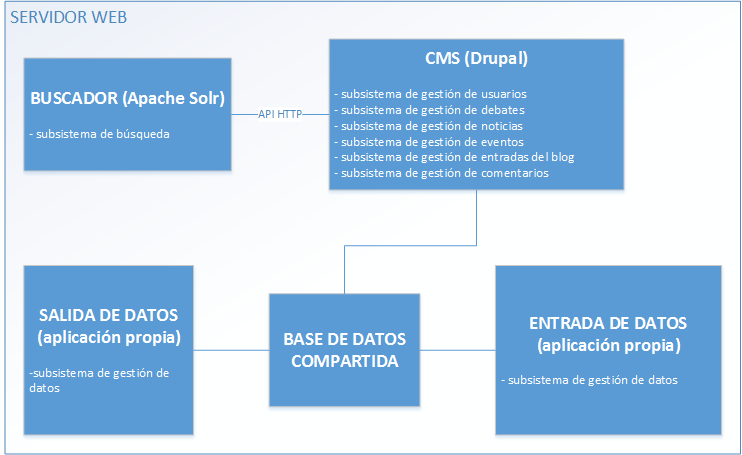
\includegraphics[width=\textwidth]{diagrama_subsistemas.png}
\caption{Diagrama de subsistemas}
\label{fig:diagrama_subsistemas}
\end{figure}


\section{Especificación de casos de uso}
\label{especificacion_casos_uso}
En esta sección se detallarán los casos de uso del sistema.  Para facilitar la lectura, los casos de uso y escenarios se agruparán por subsistemas.

Cada caso de uso tendrá la siguiente información:
\begin{itemize}
\item Nombre.  Nombre que permita identificar al caso de uso.
\item Precondiciones.  Las precondiciones indican una situación que es de obligado cumplimiento antes del caso de uso.  Por simplicidad, las precondiciones se omitirán en los casos de uso en los que no existan.
\item Descripción.  La descripción indica de forma resumida la finalidad del caso de uso.
\item Actores.  Los actores serán todos aquellos posibles participantes en el caso de uso.
\item Escenario principal.  El escenario principal indica de forma ordenada los pasos que se realizan en el caso de uso.
\item Escenarios alternativos.  Los escenarios alternativos representan variaciones o divergencias respecto al escenario principal.  Por simplicidad, los escenarios alternativos se omitirán en los casos de uso en los que no existan.
\end{itemize}


\subsection{Subsistema de gestión de usuarios}
\label{casos_uso_subsistema_usuarios}
En esta sección se detallarán los casos de uso y escenarios pertenecientes al subsistema de gestión de usuarios.
La figura \ref{fig:casos_uso_subsistema_usuarios} muestra el diagrama de casos de dicho subsistema.

\begin{figure}[h]
\centering
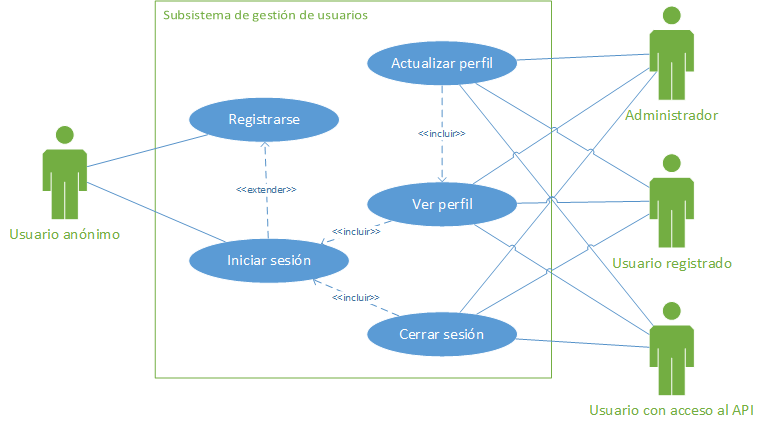
\includegraphics[width=\textwidth]{casos_uso_usuarios.png}
\caption{Diagrama de casos de uso del subsistema de gestión de usuarios}
\label{fig:casos_uso_subsistema_usuarios}
\end{figure}


\subsubsection{Caso de uso ``registrarse''}
\begin{description}
\item[Descripción] 				El usuario no dispone de una cuenta en el sistema y quiere crear una.
\item[Actores]					Cualquier usuario anónimo.
\item[Escenario principal]	 	\hfill
								\begin{enumerate}
								\item El usuario accede al formulario de registro.
								\item Una vez en el formulario de registro, el usuario rellena todos los campos requeridos.
								\item Si el usuario lo decide también puede rellenar los campos opcionales.
								\item Tras rellenar los campos el usuario pulsa el botón de registro.
								\item El sistema guarda los datos y crea la nueva cuenta de usuario con estado bloqueado.
								\end{enumerate}
\item[Escenario alternativo 1]	El usuario no rellena todos los campos necesarios.
								\begin{enumerate}
								\item Cuando el usuario pulse el botón para completar el registro el sistema notificará del error.
								\item Se continuará desde el punto 2 del escenario principal.
								\end{enumerate}
\item[Escenario alternativo 2]	El nombre de usuario ya existe en el sistema.
								\begin{enumerate}
								\item Cuando el usuario pulse el botón para completar el registro el sistema notificará del error.
								\item Se continuará desde el punto 2 del escenario principal.
								\end{enumerate}
\item[Escenario alternativo 3]	El email de usuario ya existe en el sistema.
								\begin{enumerate}
								\item Cuando el usuario pulse el botón para completar el registro el sistema notificará del error.
								\item Se continuará desde el punto 2 del escenario principal.
								\end{enumerate}
\end{description}


\subsubsection{Caso de uso ``activar usuario''}
\begin{description}
\item[Descripción] 				El administrador activa una cuenta de un usuario para que éste pueda utilizarla.
\item[Actores]					El administrador del sistema.
\item[Precondiciones]			La cuenta de usuario debe ser registrada previamente en el sistema.
\item[Escenario principal]	 	\hfill
								\begin{enumerate}
								\item El administrador accede al panel de administración.
								\item Una vez en el panel de administración, accede a la vista de usuarios.
								\item El administrador selecciona el usuario o usuarios a activar.
								\item Pulsa el botón correspondiente para activar los usuarios.
								\item El sistema actualiza el estado de los usuarios y permite que inicien sesión en el sistema.
								\end{enumerate}
\end{description}


\subsubsection{Caso de uso ``iniciar sesión''}
\begin{description}
\item[Descripción] El usuario accede al sistema utilizando su nombre de usuario y contraseña.
\item[Actores] Cualquier usuario anónimo.
\item[Precondiciones] La cuenta de usuario con la que se inicia sesión ha sido activada por un administrador.
\item[Escenario principal] \hfill
						 	\begin{enumerate}
							\item El usuario accede al formulario de inicio de sesión
							\item El usuario introduce su nombre de usuario
							\item El usuario introduce su contraseña
							\item El usuario inicia sesión pulsando el botón correspondiente
							\end{enumerate}
\item[Escenario alternativo 1] El usuario no existe
							\begin{enumerate}
							\item El sistema notificará al usuario de que el nombre de usuario introducido no existe
							\item Se continuará desde el paso 2 del escenario principal
							\end{enumerate}
\item [Escenario alternativo 2] La contraseña es incorrecta
							\begin{enumerate}
							\item El sistema notificará al usuario de que la contraseña introducida es incorrecta
							\item Se continuará desde el paso 2 del escenario principal
							\end{enumerate}							
\end{description}


\subsubsection{Caso de uso ``cerrar sesión''}
\begin{description}
\item[Descripción] 			El usuario quiere cerrar su sesión en el sistema.
\item[Actores] 				Administrador, usuario registrado o usuario con capacidad de acceso al API.
\item[Precondiciones]  		Haber iniciado sesión en el sistema
\item[Escenario principal] 	\hfill
						 	\begin{enumerate}
							\item El usuario con sesión iniciada pulsa en el botón para cerrar sesión.
							\item El sistema redirige al usuario a la vista principal con la sesión ya cerrada.
							\end{enumerate}							
\end{description}


\subsubsection{Caso de uso ``ver perfil''}
\begin{description}
\item[Descripción] 			El usuario quiere ver la información sobre su cuenta almacenada en el sistema.
\item[Actores] 				Administrador, usuario registrado o usuario con capacidad de acceso al API.
\item[Precondiciones]  		Haber iniciado sesión en el sistema
\item[Escenario principal] 	\hfill
						 	\begin{enumerate}
							\item El usuario con sesión iniciada pulsa en el botón para ver su información.
							\item El sistema muestra una vista de la cuenta del usuario con todos los datos almacenados.
							\end{enumerate}
\item[Escenario alternativo 1] El usuario cuenta con capacidad de acceso al API
							\begin{enumerate}
							\item Similar al escenario principal, pero el sistema mostrará también el \textit{token} de acceso al API.
							\end{enumerate}
\item [Escenario alternativo 2] Acceso a un perfil no propio.
							\begin{enumerate}
							\item El usuario pulsa en el perfil de otro usuario del sistema.
							\item El sistema muestra una vista de la cuenta de usuario.
							\item El sistema no muestra en ningún caso el \textit{token} de acceso al API.
							\end{enumerate}							
\end{description}


\subsubsection{Caso de uso ``actualizar perfil''}
\begin{description}
\item[Descripción] 			El usuario quiere modificar la información almacenada en el sistema sobre su cuenta.
\item[Actores] 				Administrador, usuario registrado o usuario con capacidad de acceso al API.
\item[Precondiciones]  		Haber iniciado sesión en el sistema
\item[Escenario principal] 	\hfill
						 	\begin{enumerate}
							\item El usuario con sesión iniciada pulsa en el botón para ver su información.
							\item Una vez en la vista del perfil, el usuario pulsa el botón para modificar su información.
							\item El usuario modifica los datos que considere necesarios.
							\item El usuario introduce su contraseña actual para asegurar su identidad.
							\item El sistema actualiza la información de la cuenta de usuario.
							\end{enumerate}
\item[Escenario alternativo 1] La contraseña actual no es válida.
							\begin{enumerate}
							\item El sistema informará al usuario de su error y no modificará la información almacenada.
							\item Se continua desde el punto 3 del escenario principal.
							\end{enumerate}
\item [Escenario alternativo 2] El usuario quiere modificar su contraseña.
							\begin{enumerate}
							\item El usuario debe introducir su nueva contraseña dos veces para evitar errores.
							\item Se continua desde el punto 4 del escenario principal.
							\end{enumerate}							
\item [Escenario alternativo 3] Las nuevas contraseñas no coinciden.
							\begin{enumerate}
							\item Las nuevas contraseñas introducidas no coinciden.
							\item El sistema informa al usuario del error.
							\item Se continua desde el punto 1 del escenario alternativo 2.
							\end{enumerate}							
\item[Escenario alternativo 4] El nuevo correo es inválido o ya existe en el sistema.
							\begin{enumerate}
							\item El sistema informará al usuario de su error y no modificará la información almacenada.
							\item Se continua desde el punto 3 del escenario principal.
							\end{enumerate}							
\end{description}

\subsection{Subsistema de gestión de debates}
\label{casos_uso_subsistema_debates}
En esta sección se detallarán los casos de uso y escenarios pertenecientes al subsistema de gestión de debates.
La figura \ref{fig:casos_uso_subsistema_debates} muestra el diagrama de casos de uso del subsistema de gestión de debates.

\begin{figure}[h]
\centering
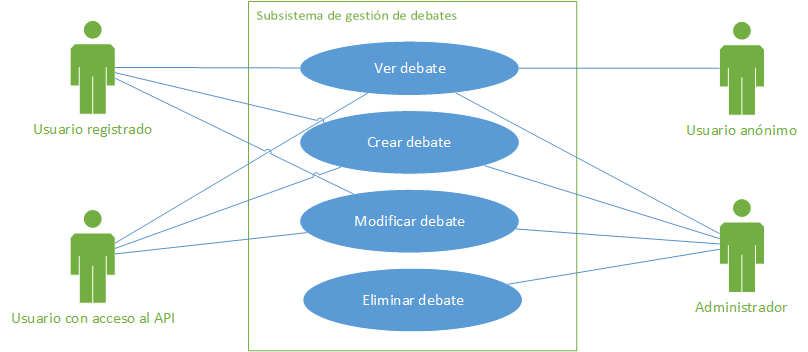
\includegraphics[width=\textwidth]{casos_uso_debates.png}
\caption{Diagrama de casos de uso del subsistema de gestión de debates}
\label{fig:casos_uso_subsistema_debates}
\end{figure}


\subsubsection{Caso de uso ``ver debate''}
\begin{description}
\item[Descripción] 				El usuario quiere ver el contenidos y los comentarios de un debate.
\item[Actores]					Cualquier usuario registrado o no en el sistema.
\item[Escenario principal]	 	\hfill
								\begin{enumerate}
								\item El usuario pulsa en el botón que carga la vista de los debates.
								\item Una vez en la vista de debates, elige el debate del que quiere ver sus contenidos.
								\item El usuario pulsa en el título del debate elegido.
								\item El sistema carga la vista del debate mostrando tanto el contenido como los comentarios del mismo.
								\end{enumerate}
\item[Escenario alternativo 1]	El usuario utiliza la búsqueda para localizar el debate.
								\begin{enumerate}
								\item El usuario accede a la vista de la búsqueda.
								\item El usuario escribe algunas palabras que se encuentren en el debate que quiere visualizar.
								\item En la lista de resultados selecciona el debate que desee.
								\item Se continua desde el punto 4 del escenario principal.
								\end{enumerate}
\end{description}


\subsubsection{Caso de uso ``crear debate''}
\begin{description}
\item[Descripción] El usuario quiere crear un nuevo debate para que puedan participar el resto de usuarios.
\item[Actores] Administrador, usuario registrado o usuario con capacidad de acceso al API.
\item[Precondiciones] Haber iniciado sesión en el sistema.
\item[Escenario principal] \hfill
						 	\begin{enumerate}
							\item El usuario accede a la vista de debates.
							\item Pulsa el botón para crear un debate.
							\item Rellena los campos requeridos en el formulario de creación del debate.
							\item Rellena los campos opcionales que considere necesarios en el formulario de creación del debate.
							\item Pulsa el botón para guardar el debate.
							\item El sistema guarda el debate con estado ``próximamente''.
							\end{enumerate}
\item[Escenario alternativo 1] El usuario no ha rellenado todos los campos requeridos.
							\begin{enumerate}
							\item El sistema notificará al usuario de que faltan campos por rellenar.
							\item Se continuará desde el punto 3 del escenario principal.
							\end{enumerate}
\end{description}


\subsubsection{Caso de uso ``comentar un debate''}
\begin{description}
\item[Descripción] El usuario quiere crear dar su opinión en un debate abierto.
\item[Actores] Administrador, usuario registrado o usuario con capacidad de acceso al API.
\item[Precondiciones] Haber iniciado sesión en el sistema.
\item[Escenario principal] \hfill
						 	\begin{enumerate}
							\item El usuario accede a la vista de debates.
							\item Selecciona el debate en el que quiere crear un comentario.
							\item Una vez en la vista del debate, el usuario escribe su comentario.
							\item Pulsa el botón de para guardar su comentario.
							\end{enumerate}
\item[Escenario alternativo 1] El usuario quiere añadir un comentario como respuesta a otro comentario ya existente.
							\begin{enumerate}
							\item Los dos primeros pasos serán similares a los del escenario principal.
							\item Una vez en la vista de debate el usuario localiza el comentario al que quiere responder y pulsa el botón correspondiente.
							\item El usuario escribe su comentario.
							\item Pulsa el botón para guardar el comentario.
							\end{enumerate}
\end{description}


\subsubsection{Caso de uso ``modificar comentario''}
\begin{description}
\item[Descripción] El usuario quiere crear modificar un comentario que ha creado previamente.
\item[Actores] Administrador, usuario registrado o usuario con capacidad de acceso al API.
\item[Precondiciones] Haber iniciado sesión en el sistema.
\item[Escenario principal] \hfill
						 	\begin{enumerate}
							\item El usuario accede a la vista de debates.
							\item Selecciona el debate en el que ha realizado el comentario que quiere modificar.
							\item Una vez en la vista del debate busca su comentario y pulsa el botón destinado a modificarlo.
							\item Introduce el nuevo texto del comentario
							\item Pulsa el botón de para guardar su comentario.
							\end{enumerate}
\end{description}


\subsubsection{Caso de uso ``moodificar debate''}
\begin{description}
\item[Descripción] Un usuario quiere modificar el contenido de un debate.
\item[Actores] Administrador, usuario registrado o usuario con capacidad de acceso al API.
\item[Precondiciones] Haber iniciado sesión en el sistema.
\item[Escenario principal] \hfill
						 	\begin{enumerate}
							\item El usuario accede a la vista de debates.
							\item Selecciona el debate cuyo contenido desea modificar.
							\item Una vez en la vista del debate pulsa el botón destinado a modificarlo.
							\item Modifica la información que sea necesaria (excepto el estado del debate, el proceso de modificación del estado de un debate está descrito en el escenario alternativo 1).
							\item Pulsa el botón de para guardar las modificaciones.
							\item El sistema actualiza los contenidos del debate.
							\end{enumerate}
\item[Escenario alternativo 1]  Modificar el estado de un debate.
							\begin{enumerate}
							\item El administrador accede al panel de administración.
							\item Selecciona el debate que desea modificar y pulsa el botón correspondiente.
							\item En la vista de edición del debate selecciona el nuevo estado que desea asignarle.
							\item Se continúa desde el punto 5 del escenario principal.
							\end{enumerate}
\item[Escenario alternativo 2]  No se rellenan todos los campos requeridos
							\begin{enumerate}
							\item El sistema informa al usuario del error y no modifica la información almacenada.
							\item Se continúa desde el punto 4 del escenario principal.
							\end{enumerate}
\end{description}


\subsubsection{Caso de uso ``eliminar debate''}
\begin{description}
\item[Descripción] El administrador quiere eliminar un debate junto con todos sus comentarios.
\item[Actores] Administrador.
\item[Precondiciones] Haber iniciado sesión en el sistema.
\item[Escenario principal] \hfill
						 	\begin{enumerate}
							\item El administardor accede a la vista de administración.
							\item Localiza el debate que desea eliminar y pulsa el botón correspondiente.
							\item El debate y sus comentarios serán eliminados del sistema.
							\end{enumerate}
\end{description}

\subsection{Subsistema de gestión de eventos}
\label{casos_uso_subsistema_eventos}
En esta sección se detallarán los casos de uso pertenecientes al subsistema de gestión de eventos. La figura \ref{fig:casos_uso_subsistema_eventos} muestra el diagrama de casos de uso de dicho subsistema.

\begin{figure}[h]
\centering
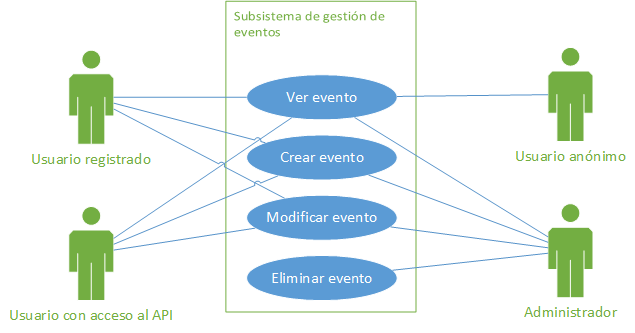
\includegraphics[width=\textwidth]{casos_uso_eventos}
\caption{Diagrama de casos de uso del subsistema de gestión de eventos}
\label{fig:casos_uso_subsistema_eventos}
\end{figure}


\subsubsection{Caso de uso ``ver evento''}
\begin{description}
\item[Descripción] Un usuario quiere ver el contenido de un evento.
\item[Actores] Cualquier usuario registrado o no en el sistema.
\item[Escenario principal] 	\hfill
							\begin{enumerate}
							\item El usuario accede a la vista de eventos.
							\item Una vez en la vista de eventos, elige el evento del que quiere ver sus contenidos.
							\item Pulsa en el título del evento que quiere ver en detalle.
							\item El sistema carga la vista del evento mostrando todos sus detalles.
							\end{enumerate}
\end{description}


\subsubsection{Caso de uso ``crear evento''}
\begin{description}
\item[Descripción]  Un usuario quiere añadir un nuevo evento al sistema.
\item[Actores]  Administrador, usuario registrado o usuario con capacidad de acceso al API.
\item[Precondiciones] Haber iniciado sesión en el sistema.
\item[Escenario principal]  \hfill
							\begin{enumerate}
							\item El usuario accede a la vista de los eventos.
							\item Una vez en la vista de eventos pulsa el botón correspondiente para crear un evento nuevo.
							\item Rellena el formulario con los datos requeridos.
							\item Si lo desea también rellena la información opcional del formulario.
							\item El usuario pulsa el botón guardar, y el sistema crea el nuevo evento.
							\end{enumerate}
\item[Escenario alternativo 1] No se han rellenado todos los campos requeridos.
							\begin{enumerate}
							\item El usuario no ha rellenado todos los campos requeridos para crear un nuevo evento.
							\item El sistema notificará al usuario de su error y no creará el nuevo evento.
							\item Se continuará desde el punto 3 del escenario principal.
							\end{enumerate}
\end{description}


\subsubsection{Caso de uso ``modificar evento''}
\begin{description}
\item[Descripción]  Un usuario quiere modificar un evento del sistema.
\item[Actores]  Administrador, usuario registrado o usuario con capacidad de acceso al API.
\item[Precondiciones]  Haber iniciado sesión en el sistema.
\item[Escenario principal]	\hfill
							\begin{enumerate}
							\item El usuario accede a la vista de los eventos..
							\item Una vez en la vista de eventos localiza el evento que quiere modificar.
							\item Cuando ha accedido al evento pulsa el botón correspondiente para modificar su contenido.
							\item Rellena toda la información requerida en el formulario.
							\item Si lo desea también rellena la información opcional del formulario.
							\item El usuario pulas el botón guardar y el sistema modifica la información del evento.
							\end{enumerate}
\item[Escenario alternativo 1] No se han rellenado todos los campos requeridos.
							\begin{enumerate}
							\item El usuario no ha rellenado todos los campos requeridos para modificar el evento.
							\item El sistema notificará al usuario de su error y no modificará los datos del evento.
							\item Se continuará desde el punto 4 del escenario principal.
							\end{enumerate}
\end{description}


\subsubsection{Caso de uso ``eliminar evento''}
\begin{description}
\item[Descripción]  Un administrador quiere eliminar un evento del sistema.
\item[Actores] El administrador del sistema.
\item[Precondiciones]  Haber iniciado sesión en el sistema.
\item[Escenario principal]	\hfill
							\begin{enumerate}
							\item El administrador accede a la vista de administración.
							\item Localiza el evento que desea eliminar y pulsa el botón correspondiente.
							\item El evento será eliminado del sistema.
							\end{enumerate}
\end{description}

\subsection{Subsistema de gestión de noticias}
\label{casos_uso_subsistema_noticias}
En esta sección se detallarán los casos de uso pertenecientes al subsistema de gestión de noticias. La figura \ref{fig:casos_uso_subsistema_noticias} muestra el diagrama de casos de uso de dicho subsistema.

\begin{figure}[h]
\centering
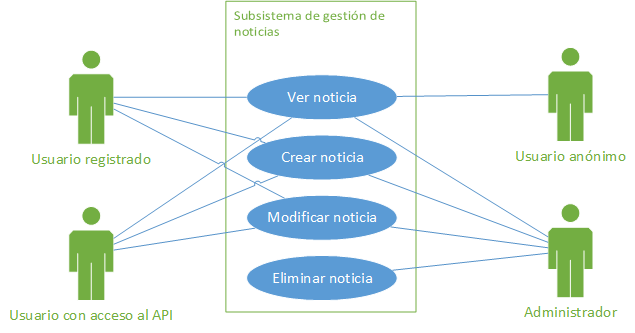
\includegraphics[width=\textwidth]{casos_uso_noticias}
\caption{Diagrama de casos de uso del subsistema de gestión de noticias}
\label{fig:casos_uso_subsistema_noticias}
\end{figure}


\subsubsection{Caso de uso ``ver noticia''}
\begin{description}
\item[Descripción] Un usuario quiere ver el contenido de una noticia.
\item[Actores] Cualquier usuario registrado o no en el sistema.
\item[Escenario principal] 	\hfill
							\begin{enumerate}
							\item El usuario pulsa en el botón que carga la vista de las noticias.
							\item Una vez en la vista de noticias pulsa en el título de la noticia que quiere ver en detalle.
							\item El sistema carga la vista de la noticia mostrando todos sus detalles.
							\end{enumerate}
\end{description}


\subsubsection{Caso de uso ``crear noticia''}
\begin{description}
\item[Descripción]  Un usuario quiere añadir una nueva noticia al sistema.
\item[Actores]  Administrador, usuario registrado o usuario con capacidad de acceso al API.
\item[Precondiciones] Haber iniciado sesión en el sistema.
\item[Escenario principal]  \hfill
							\begin{enumerate}
							\item El usuario pulsa en el botón que carga la vista de las noticias.
							\item Una vez en la vista de las noticias pulsa el botón correspondiente para crear una noticia nueva.
							\item Rellena el formulario con los datos requeridos.
							\item Si lo desea también rellena la información opcional del formulario.
							\item El usuario pulsa el botón guardar.
							\item El sistema crea la nueva noticia.
							\end{enumerate}
\item[Escenario alternativo 1] No se han rellenado todos los campos requeridos.
							\begin{enumerate}
							\item El usuario no ha rellenado todos los campos requeridos para crear una nueva noticia.
							\item El sistema notificará al usuario de su error y no creará la nueva noticia.
							\item Se continuará desde el punto 3 del escenario principal.
							\end{enumerate}
\end{description}


\subsubsection{Caso de uso ``modificar noticia''}
\begin{description}
\item[Descripción]  Un usuario quiere modificar una noticia del sistema.
\item[Actores]  Administrador, usuario registrado o usuario con capacidad de acceso al API.
\item[Precondiciones]  Haber iniciado sesión en el sistema.
\item[Escenario principal]	\hfill
							\begin{enumerate}
							\item El usuario accede a la vista de las noticias.
							\item Una vez en la vista de noticias localiza la noticia que quiere modificar.
							\item Cuando ha accedido a la noticia pulsa el botón correspondiente para modificar su contenido.
							\item Rellena toda la información requerida en el formulario.
							\item Si lo desea también rellena la información opcional del formulario.
							\item El usuario pulas el botón guardar.
							\item El sistema actualiza la información de la noticia editada.
							\end{enumerate}
\item[Escenario alternativo 1] No se han rellenado todos los campos requeridos.
							\begin{enumerate}
							\item El usuario no ha rellenado todos los campos requeridos para modificar la noticia.
							\item El sistema notificará al usuario de su error y no modificará los datos la noticia.
							\item Se continuará desde el punto 4 del escenario principal.
							\end{enumerate}
\end{description}


\subsubsection{Caso de uso ``eliminar noticia''}
\begin{description}
\item[Descripción]  Un administrador quiere eliminar una noticia del sistema.
\item[Actores]  El administrador del sistema.
\item[Precondiciones]  Haber iniciado sesión en el sistema.
\item[Escenario principal]	\hfill
							\begin{enumerate}
							\item El administrador accede a la vista de administración.
							\item Localiza la noticia que desea eliminar y pulsa el botón correspondiente.
							\item La noticia será eliminado del sistema.
							\end{enumerate}
\end{description}

\subsection{Subsistema de gestión del blog}
\label{casos_uso_subsistema_blog}
En esta sección se detallarán los casos de uso y escenarios pertenecientes al subsistema de gestión de entradas del blog. La figura \ref{fig:casos_uso_subsistema_blog} muestra el diagrama de casos de uso del subsistema de gestión de debates.

\begin{figure}[h]
\centering
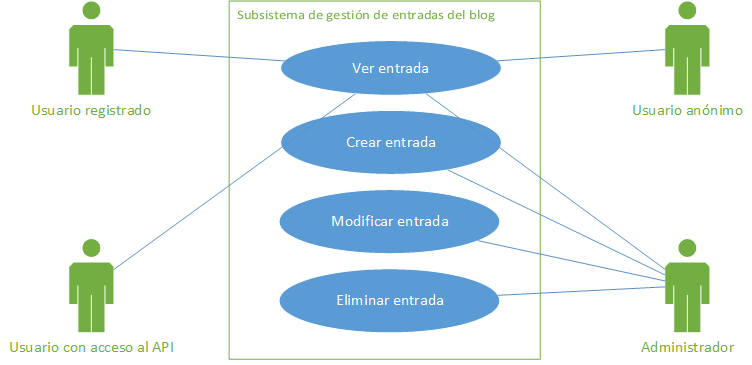
\includegraphics[width=\textwidth]{casos_uso_blog}
\caption{Diagrama de casos de uso del subsistema de gestión de entradas del blog}
\label{fig:casos_uso_subsistema_blog}
\end{figure}


\subsubsection{Caso de uso ``ver entrada''}
\begin{description}
\item[Descripción] 				El usuario quiere ver el contenido de una entrada del blog.
\item[Actores]					Cualquier rol de usuario.
\item[Escenario principal]	 	\hfill
								\begin{enumerate}
								\item El usuario accede al blog del Land Portal.
								\item Una vez en el blog, selecciona la entrada que quiere ver en detalle.
								\item El sistema carga la vista de la entrada mostrando tanto su contenido como sus comentarios.
								\end{enumerate}
\end{description}


\subsubsection{Caso de uso ``crear entrada''}
\begin{description}
\item[Descripción] El administrador quiere crear una nueva entrada en el blog del Land Portal.
\item[Actores] Administrador.
\item[Precondiciones] Haber iniciado sesión en el sistema.
\item[Escenario principal] \hfill
						 	\begin{enumerate}
							\item El administrador accede al blog del Land Portal.
							\item Una vez en el blog, el administrador pulsa el botón para crear una nueva entrada.
							\item Rellena los campos requeridos en el formulario de creación de la entrada.
							\item Rellena los campos opcionales que considere necesarios en el formulario de creación de la entrada.
							\item Pulsa el botón para guardar la entrada.
							\item El sistema guarda la entrada y la hace visible para todos los usuarios en el blog.
							\end{enumerate}
\item[Escenario alternativo 1] El administrador no ha rellenado todos los campos requeridos.
							\begin{enumerate}
							\item El sistema notificará al usuario de que faltan campos por rellenar.
							\item Se continuará desde el punto 3 del escenario principal.
							\end{enumerate}
\end{description}


\subsubsection{Caso de uso ``modificar entrada''}
\begin{description}
\item[Descripción] El administrador quiere modificar el contenido de una entrada del blog.
\item[Actores] El administrador del sistema.
\item[Precondiciones] Haber iniciado sesión en el sistema.
\item[Escenario principal] \hfill
						 	\begin{enumerate}
							\item El administrador accede al blog del Land Portal.
							\item Una vez en el blog, el administrador selecciona la entrada que quiere modificar.
							\item En la entrada correspondiente, el administrador pulsa el botón para editar su contenido.
							\item Rellena los campos requeridos en el formulario de modificación de la entrada.
							\item Rellena los campos opcionales que considere necesarios en el formulario de modificación de la entrada.
							\item Pulsa el botón para guardar los cambios
							\item El sistema actualiza los contenidos de la entrada del blog.
							\end{enumerate}
\item[Escenario alternativo 1]  No se rellenan todos los campos requeridos
							\begin{enumerate}
							\item El sistema informa al usuario del error y no modifica la información almacenada.
							\item Se continúa desde el punto 4 del escenario principal.
							\end{enumerate}
\end{description}

\subsubsection{Caso de uso ``eliminar entrada''}
\begin{description}
\item[Descripción] El administrador quiere eliminar una entrada del blog junto con todos sus comentarios.
\item[Actores] El administrador del sistema.
\item[Precondiciones] Haber iniciado sesión en el sistema.
\item[Escenario principal] \hfill
						 	\begin{enumerate}
							\item El administrador accede a la vista de administración.
							\item En la sección de contenidos localiza la entrada y pulsa el botón correspondiente para eliminarla.
							\item La entrada y sus comentarios serán eliminados del sistema.
							\end{enumerate}
\end{description}



\subsection{Subsistema de gestión de comentarios}
\label{casos_uso_subsistema_comentarios}
En esta sección se detallarán los casos de uso y escenarios pertenecientes al subsistema de gestión de comentarios. La figura \ref{fig:casos_uso_subsistema_comentarios} muestra el diagrama de casos de uso de dicho subsistema.

\begin{figure}[h]
\centering
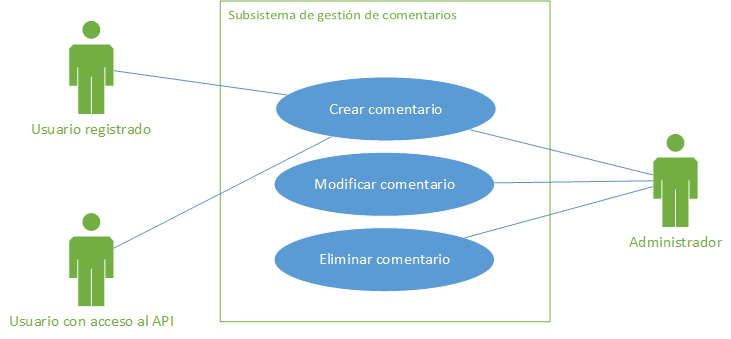
\includegraphics[width=\textwidth]{casos_uso_comentarios}
\caption{Diagrama de casos de uso del subsistema de gestión de comentarios}
\label{fig:casos_uso_subsistema_comentarios}
\end{figure}


\subsubsection{Caso de uso ``crear comentario''}
\begin{description}
\item[Descripción] El usuario quiere crear un nuevo comentario.
\item[Actores] Administrador, usuario registrado o usuario con capacidad de acceso al API.
\item[Precondiciones] Haber iniciado sesión en el sistema.
\item[Escenario principal] \hfill
						 	\begin{enumerate}
							\item El usuario accede a la entrada del blog o al debate en el que quiere crear el comentario.
							\item El usuario escribe su comentario.
							\item Pulsa el botón de para guardar su comentario.
							\item El sistema guarda el comentario y lo hace visible al resto de usuarios.
							\end{enumerate}
\item[Escenario alternativo 1] Comentario en un  debate cerrado.
							\begin{enumerate}
							\item El usuario accede al debate en el que quiere crear el comentario.
							\item El sistema no mostrará opciones para que el usuario cree un comentario.
							\end{enumerate}
\end{description}


\subsubsection{Caso de uso ``modificar comentario''}
\begin{description}
\item[Descripción] El administrador desea modificar el contenido de un comentario realizado por un usuario.
\item[Actores] Administrador.
\item[Precondiciones] Haber iniciado sesión en el sistema.
\item[Escenario principal] \hfill
						 	\begin{enumerate}
							\item El usuario accede a la entrada del blog o al debate en el que se encuentra el comentario a modificar.
							\item El administrador localiza el comentario y pulsa el botón modificar.
							\item El administrador introduce el texto que crea conveniente y pulsa el botón guardar.
							\item El sistema actualiza el contenido del comentario modificado.
							\end{enumerate}
\end{description}


\subsubsection{Caso de uso ``eliminar comentario''}
\begin{description}
\item[Descripción] El administrador desea eliminar un comentario realizado por un usuario.
\item[Actores] Administrador.
\item[Precondiciones] Haber iniciado sesión en el sistema.
\item[Escenario principal] \hfill
						 	\begin{enumerate}
							\item El usuario accede a la entrada del blog o al debate en el que se encuentra el comentario a eliminar.
							\item El administrador localiza el comentario y pulsa el botón eliminar.
							\item El sistema elimina el comentario y deja de mostrarlo.
							\end{enumerate}
\end{description}

\subsection{Subsistema de gestión de organizaciones}
\label{casos_uso_subsistema_organizaciones}
En esta sección se detallarán los casos de uso pertenecientes al subsistema de gestión de organizaciones. La figura \ref{fig:casos_uso_subsistema_organizaciones} muestra el diagrama de casos de uso de dicho subsistema.

\begin{figure}[h]
\centering
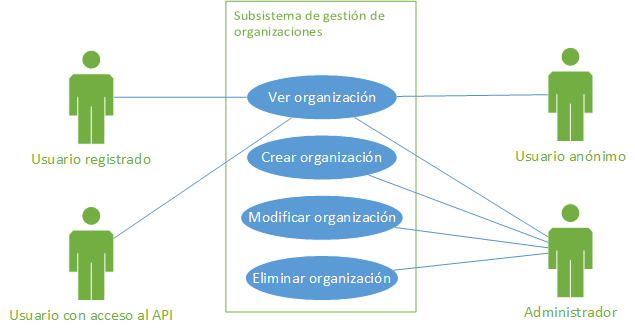
\includegraphics[width=\textwidth]{casos_uso_organizaciones}
\caption{Diagrama de casos de uso del subsistema de gestión de organizaciones}
\label{fig:casos_uso_subsistema_organizaciones}
\end{figure}


\subsubsection{Caso de uso ``ver organización''}
\begin{description}
\item[Descripción] Un usuario quiere ver la información sobre una organización.
\item[Actores] Cualquier usuario registrado o no en el sistema.
\item[Escenario principal] 	\hfill
							\begin{enumerate}
							\item El usuario pulsa en el botón que carga la vista de las organizaciones.
							\item Una vez en la vista de organizaciones pulsa en el nombre o la imagen de la organización que quiere ver en detalle.
							\item El sistema carga la vista de la organización mostrando todos sus detalles.
							\end{enumerate}
\end{description}


\subsubsection{Caso de uso ``crear organización''}
\begin{description}
\item[Descripción]  Un administrador quiere añadir una nueva organización al sistema.
\item[Actores]  El administrador del sistema.
\item[Precondiciones] Haber iniciado sesión en el sistema.
\item[Escenario principal]  \hfill
							\begin{enumerate}
							\item El usuario pulsa en el botón que carga la vista de las organizaciones.
							\item Una vez en la vista de las organizaciones pulsa el botón correspondiente para crear una organización nueva.
							\item Rellena el formulario con los datos requeridos.
							\item Si lo desea también rellena la información opcional del formulario.
							\item El administrador pulsa el botón guardar.
							\item El sistema crea la nueva noticia.
							\end{enumerate}
\item[Escenario alternativo 1] No se han rellenado todos los campos requeridos.
							\begin{enumerate}
							\item El administrador no ha rellenado todos los campos requeridos para crear una nueva organización.
							\item El sistema notificará al administrador de su error y no creará la nueva organización.
							\item Se continuará desde el punto 3 del escenario principal.
							\end{enumerate}
\end{description}


\subsubsection{Caso de uso ``modificar organización''}
\begin{description}
\item[Descripción]  Un administrador quiere modificar una organización existente en el sistema.
\item[Actores]  El administrador del sistema.
\item[Precondiciones] Haber iniciado sesión en el sistema.
\item[Escenario principal]	\hfill
							\begin{enumerate}
							\item El usuario accede a la vista de las organizaciones.
							\item Una vez en la vista de noticias localiza la organización que quiere modificar.
							\item Cuando ha accedido a la organización pulsa el botón correspondiente para modificar su contenido.
							\item Rellena toda la información requerida en el formulario.
							\item Si lo desea también rellena la información opcional del formulario.
							\item El administrador pulsa el botón guardar.
							\item El sistema actualiza la información de la organización editada.
							\end{enumerate}
\item[Escenario alternativo 1] No se han rellenado todos los campos requeridos.
							\begin{enumerate}
							\item El administrador no ha rellenado todos los campos requeridos para modificar la organización.
							\item El sistema notificará al usuario de su error y no modificará los datos de la organización.
							\item Se continuará desde el punto 4 del escenario principal.
							\end{enumerate}
\end{description}


\subsubsection{Caso de uso ``eliminar organización''}
\begin{description}
\item[Descripción]  Un administrador quiere eliminar una organización del sistema.
\item[Actores]  El administrador del sistema.
\item[Precondiciones]  Haber iniciado sesión en el sistema.
\item[Escenario principal]	\hfill
							\begin{enumerate}
							\item El administrador accede a la vista de las organizaciones.
							\item Accede a la organización que desea eliminar.
							\item Una vez en la vista de la organización pulsa el botón correspondiente para su eliminación.
							\item La organización será eliminada del sistema.
							\end{enumerate}
\end{description}

\subsection{Subsistema de búsqueda}
\label{casos_uso_subsistema_busqueda}
En esta sección se detallarán los casos de uso y escenarios pertenecientes al subsistema de búsqueda. La figura \ref{fig:casos_uso_subsistema_busqueda} muestra el diagrama de casos de uso de dicho subsistema.

\begin{figure}[h]
\centering
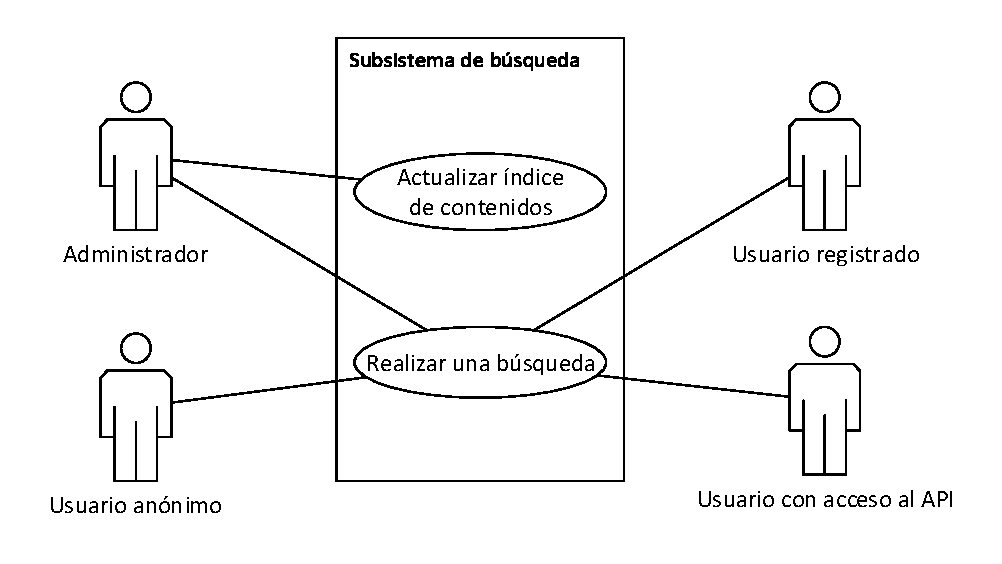
\includegraphics[width=\textwidth]{casos_uso/diagrama_casos_uso_busqueda}
\caption{Diagrama de casos de uso del subsistema de búsqueda}
\label{fig:casos_uso_subsistema_busqueda}
\end{figure}

\subsubsection{Caso de uso ``realizar una búsqueda''}
\begin{description}
\item[Descripción] Un usuario busca información en el sistema.
\item[Actores] Cualquier rol de usuario registrado o no en el sistema.
\item[Escenario principal] \hfill
							\begin{enumerate}
							\item El usuario introduce un texto en el formulario de búsqueda
							\item El usuario pulsa el botón de buscar
							\item El sistema devuelve los resultados correspondientes
							\end{enumerate}						
\end{description}

\subsubsection{Caso de uso ``actualizar índice de contenidos''}
\begin{description}
\item[Descripción] El administrador actualiza el índice de contenidos del subsistema de búsqueda.
\item[Actores] El administrador del sistema.
\item[Escenario principal] \hfill
							\begin{enumerate}
							\item El administrador accede al panel de administración.
							\item Una vez en el panel de administración, accede a las opciones de la búsqueda
							\item El administrador pulsa el botón correspondiente para realizar la regeneración del índice de contenidos.
							\item El sistema actualiza el índice de contenidos incluyendo los nuevos contenidos y eliminado los contenidos que ya no existan.
							\end{enumerate}						
\end{description}

\subsection{Subsistema de gestión de datos}
\label{casos_uso_subsistema_datos}
En esta sección se detallarán los casos de uso pertenecientes al subsistema de datos. La figura \ref{fig:casos_uso_subsistema_datos} muestra el diagrama de casos de uso de dicho subsistema.

\begin{figure}[h]
\centering
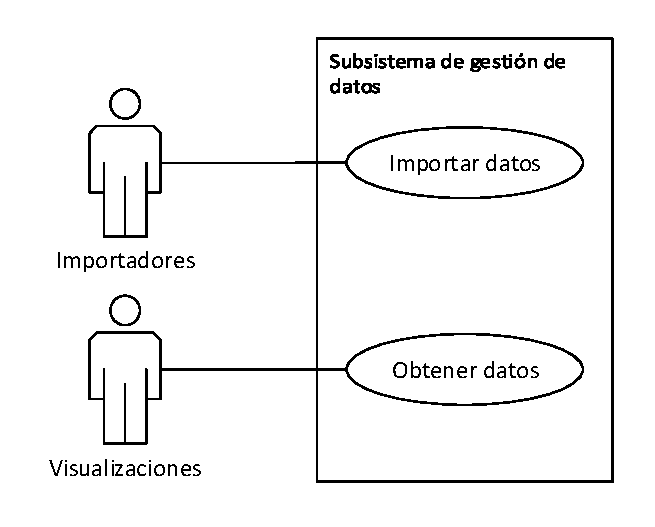
\includegraphics{casos_uso/diagrama_casos_uso_datos}
\caption{Diagrama de casos de uso del subsistema de datos}
\label{fig:casos_uso_subsistema_datos}
\end{figure}

\subsubsection{Caso de uso ``importar datos''}
\begin{description}
\item[Descripción] Un importador quiere incluir nueva información en el sistema.
\item[Actores] Un importador.
\item[Escenario principal] \hfill
							\begin{enumerate}
							\item El importador envía una petición POST al subsistema de datos incluyendo un fichero XML conforme a un XML Schema definido y con los datos a incluir en el sistema.
							\item El subsistema de datos comprueba si la dirección de origen de la petición está en la lista blanca.
							\item El subsistema de datos procesa la petición convirtiendo la información del fichero XML a un modelo propio.
							\item El subsistema de datos persiste en la base de datos el modelo creado anteriormente.
							\item El subsistema envía una respuesta 200 (\textit{OK}) al importador.
							\end{enumerate}
\item[Escenario alternativo 1] Los datos enviados por el importador no se ajustan al XML Schema.
							\begin{enumerate}
							\item El subsistema de datos no insertará ningún dato en la base de datos.
							\item El subsistema de datos envía una respuesta de error al importador.
							\end{enumerate}
\item[Escenario alternativo 2] El verbo utilizado por el importador no es el correcto (GET, PUT, etc).
							\begin{enumerate}
							\item El subsistema de datos no insertará ningún dato en la base de datos.
							\item El subsistema de datos envía una respuesta de error 405 (\textit{Method not Allowed}) al importador.
							\end{enumerate}
\item[Escenario alternativo 3] La petición realizada por el importador no incluye el fichero XML con los datos.
							\begin{enumerate}
							\item El subsistema de datos no insertará ningún dato en la base de datos.
							\item El subsistema de datos envía una respuesta de error 400 (\textit{Bad Request}) al importador.
							\end{enumerate}
\item[Escenario alternativo 4] La petición proviene de un origen no confiable
							\begin{enumerate}
							\item El subsistema de datos aborta la petición con un código de error 403 (\textit{Forbidden}).
							\end{enumerate}
\end{description}	

\subsubsection{Caso de uso ``obtener datos''}
\begin{description}
\item[Descripción] Una visualización pide datos para presentarlos al usuario de forma atractiva.
\item[Actores] Visualizaciones.
\item[Escenario principal] 	\hfill
							\begin{enumerate}
							\item La visualización lanza una petición GET al subsistema de datos.
							\item El subsistema de datos devuelve un fichero JSON con los datos correspondientes a la petición realizada.
							\item La visualización procesa los datos recibidos para presentarlos de forma visual.
							\end{enumerate}
\item[Escenario alternativo 1] La petición de la visualización es errónea.
							\begin{enumerate}
							\item La visualización lanza una petición al subsistema de datos.
							\item El subsistema de datos responde con un código de error HTTP.
							\end{enumerate}
\end{description}


\section{Clases preliminares del modelo}
\label{clases_preliminares_modelo}
En esta sección se realizará un análisis preliminar de las clases del sistema.  El objetivo de este análisis será mostrar una primera versión de los datos del modelo del sistema y de sus relaciones.

Para facilitar la lectura, se dividirá el análisis de clases en dos partes: una parte contendrá las clases pertenecientes a la zona social y la otra parte contendrá las clases pertenecientes a la zona de datos.


\subsection{Análisis preliminar de clases de la zona de datos}
\label{clases_preliminares_modelo_datos}
A continuación se realizará el análisis de las clases pertenecientes a la zona de datos. Como se ha explicado anteriormente en la sección \nameref{identificacion_subsistemas} perteneciente al capítulo \ref{chapter04}, la zona de datos incluye únicamente el subsistema de datos, que será el encargado de introducir datos en el sistema y devolverlos cuando sean pedidos por las visualizaciones.

La figura \ref{fig:clases_preliminares_modelo_book} muestra el diagrama de las clases preliminares de la zona datos.

\begin{landscape}
	\begin{figure}[ht]
		\centering
		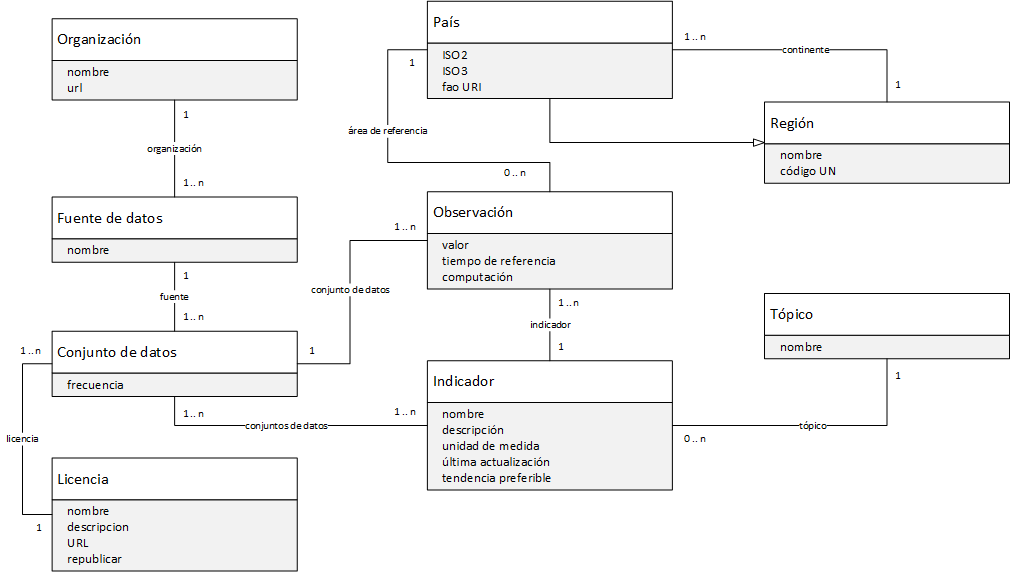
\includegraphics[height=\textwidth]{clases/clases_book_preliminar}
		\caption{Diagrama de clases preliminares de la zona de datos}
		\label{fig:clases_preliminares_modelo_book}
	\end{figure}
\end{landscape}


\subsubsection{Descripción de las clases}
\begin{description}
\item[Región]	Representa un país o continente del mundo.  Sus atributos son los siguientes:
							\begin{itemize}
								\item \textbf{Nombre}  Será el nombre de la región, por ejemplo ``Europa'', ``África'' o ``España''.
								\item \textbf{Código UN}  Será el código numérico asignado por la División Estadística de las Naciones Unidas\footnote{Éste código recibe el nombre formal de ``ISO 3166-1 numeric''.  En \cite{un:standard-country-codes} y \cite{un:iso-3166-country-codes} puede encontrarse más información sobre éstos códigos.} para la región.
							\end{itemize}
\item[País]  Representa a un país del mundo sobre el que se almacenarán observaciones.  Además de los atributos de una región, sus atributos serán:
							\begin{itemize}
							\item \textbf{ISO2}  Será el código alfabético de dos letras asignado por la división estadística de las Naciones Unidas\footnote{Éste código recibe el nombre formal de ``ISO 3166-1 alpha-2''. Se utiliza para hacer representar países, territorios independientes o zonas geográficas de interés especial. En \cite{un:iso-3166-country-codes} puede encontrarse más información sobre éstos códigos} para el país.
							\item \textbf{ISO3}  Será el código alfabético de tres letras asignado por la división estadística de las Naciones Unidas\footnote{Éste código recibe el nombre formal de ``ISO 3166-1 alpha-3''. Se utiliza para hacer representar países, territorios independientes o zonas geográficas de interés especial. En \cite{un:iso-3166-country-codes} puede encontrarse más información sobre éstos códigos} para el país.  El código ISO3 consigue una mejor asociación con los nombres de los países que el código ISO2.
							\item \textbf{FAO URI}  Será la URI única del país en la Ontología Geopolítica de la Organización para la Alimentación y la Agricultura de las Naciones Unidas\footnote{La información sobre ésta ontología se encuentra disponible en \cite{fao:geopolitical-ontology}}.
							\item \textbf{Continente}  Representa el continente del que el país forma parte.  Cada país forma parte de un continente, pero un continente puede estar compuesto de muchos países.
							\end{itemize}
\item[Observación]  Representa una medición realizada en un tiempo concreto para un país determinado.  Las observaciones son utilizadas por las visualizaciones para presentar los datos de forma visual a los usuarios.  Sus atributos serán los siguientes:
							\begin{itemize}
							\item \textbf{Valor}  Será el valor concreto de la observación.
							\item \textbf{Tiempo de referencia}  Será el tiempo al que hace referencia la observación.  Por ejemplo, el tiempo de referencia puede ser un año, un mes, un intervalo de años, etc.
							\item \textbf{Computación}  Indica el tipo de computación de la que proviene la observación.  Por ejemplo indica si el valor de la observación es único o un agregado de los valores durante un determinado periodo de tiempo.
							\item \textbf{Área de referencia}  Representa el país al que la observación hace referencia.  Cada observación hace referencia a un país, pero un país puede tener muchas observaciones que le hagan referencia.
							\item \textbf{Indicador}  Representa el indicador al que pertenece la observación.  Cada observación pertenece a un indicador, pero un indicador puede contener multitud de observaciones.
							\item \textbf{Conjunto de datos}  Representa el conjunto de datos del que proviene la observación.  Cada observación proviene de un único conjunto de datos, pero cada conjunto de datos incluye múltiples observaciones.
							\end{itemize}
\item[Indicador]  Representa un elemento sobre el que se realizan observaciones.  Sus atributos son lo siguientes:
							\begin{itemize}
							\item \textbf{Nombre}  Es un nombre corto para un indicador.
							\item \textbf{Descripción}  Es una descripción sobre lo que representa el indicador.  Por ejemplo ``Índice de Desarrollo Humano''\footnote{El Índice de Desarrollo Humano (HDI) es un indicador real mantenido por el United Nations Development Programme (UNDP) y que se encontrará en la zona de datos del portal final}.
							\item \textbf{Unidad de medida}  Representa la unidad de medida de las observaciones del indicador.  Por ejemplo el indicador ``propiedad de las tierras por parte de mujeres'' podría tener una unidad de medida en porcentaje.
							\item \textbf{Última actualización}  Indica la fecha de la última actualización del indicador o alguna de sus observaciones en el sistema.
							\item \textbf{Tendencia preferible}  Representa si es preferible que el valor del indicador crezca o disminuya a lo largo del tiempo.  Por ejemplo para el indicador ``mortalidad infantil'' la tendencia preferible será que disminuya.
							\item \textbf{Tópico}  Representa el tópico (categoría) en la que se incluye el indicador.  Cada indicador pertenece a un tópico, pero un tópico puede tener muchos indicadores relacionados.
							\item \textbf{Conjuntos de datos}  Representa los conjuntos de datos en los que el indicador está presente.  Un indicador puede estar presente en muchos conjuntos de datos y, al mismo tiempo, un conjunto de datos puede contener muchos indicadores diferentes.
							\end{itemize}
\item[Tópico]  Representa un categoría de indicadores que tratan sobre un mismo tema.  Sus atributos son lo siguientes:
							\begin{itemize}
							\item \textbf{Nombre}  Es el nombre del tópico.  Por ejemplo ``Tierra y género'' o ``Propiedad de la tierra''.
							\end{itemize}
\item[Conjunto de datos]  Representa un conjunto de datos que se inserta en el sistema.  Sus atributos son los siguientes:
							\begin{itemize}
							\item \textbf{Frecuencia}  Indica la frecuencia con la que se actualiza el conjunto de datos.  Algunas frecuencias de ejemplo pueden ser: ``anual'', ``trimestral'', etc.
							\item \textbf{Fuente}  Representa la fuente de la que proviene el conjunto de datos.  Cada conjunto de datos pertenece a una fuente, pero cada fuente puede contener varios conjuntos de datos.
							\item \textbf{Licencia}  Representa la licencia bajo la que se publica el conjunto de datos.  Cada conjunto de datos se publica bajo una licencia, pero cada licencia puede tener varios conjuntos de datos.
							\end{itemize}
\item[Licencia]  Representa una licencia bajo la que se publica un conjunto de datos.  Sus atributos son los siguientes:
							\begin{itemize}
							\item \textbf{Nombre}  Es el nombre corto de la licencia,  Por ejemplo  ``CC BY 2.0''.
							\item \textbf{Descripción}  Es una descripción larga sobre el funcionamiento de la licencia.
							\item \textbf{URL}  Será la URL bajo la que se encuentra disponible la información de la licencia  Por ejemplo \url{https://creativecommons.org/licenses/by/2.0/} para la licencia ``CC BY 2.0''.
							\item \textbf{Republicar}  Indica si la licencia permite republicar los contenidos o no.
							\end{itemize}
\item[Fuente de datos] Representa una fuente de datos de la que se extraen conjuntos de datos.  Sus atributos son los siguientes:
							\begin{itemize}
							\item \textbf{Nombre}  Es el nombre de la fuente de datos.  Por ejemplo ``Indicadores sobre el hambre''.
							\end{itemize}
\item[Organización]  Representa una organización que provee fuentes y conjuntos de datos que se importan en el sistema:
							\begin{itemize}
							\item \textbf{Nombre}  Es el nombre de la organización.  Por ejemplo  ``The Statistics Division of the FAO''\footnote{\url{http://faostat.fao.org/}}.
							\item \textbf{URL}  Es la URL del sitio web de la organización.
							\end{itemize}
\end{description}

\subsection{Análisis preliminar de clases de la zona social}
\label{clases_preliminares_modelo_debate}
A continuación se realizará el análisis preliminar de las clases pertenecientes a la zona social del sistema.  Como se ha explicado anteriormente en la sección \nameref{identificacion_subsistemas} perteneciente al capítulo \ref{chapter04}, la zona social engloba los subsistemas de:
\begin{itemize}
	\item gestión de usuarios
	\item gestión de debates
	\item gestión de eventos
	\item gestión de noticias
	\item gestión de entradas del blog
	\item gestión de comentarios
\end{itemize}

La figura \ref{fig:clases_preliminares_modelo_debate} muestra el diagrama de las clases preliminares de la zona social.

\begin{landscape}
	\begin{figure}[ht]
		\centering
		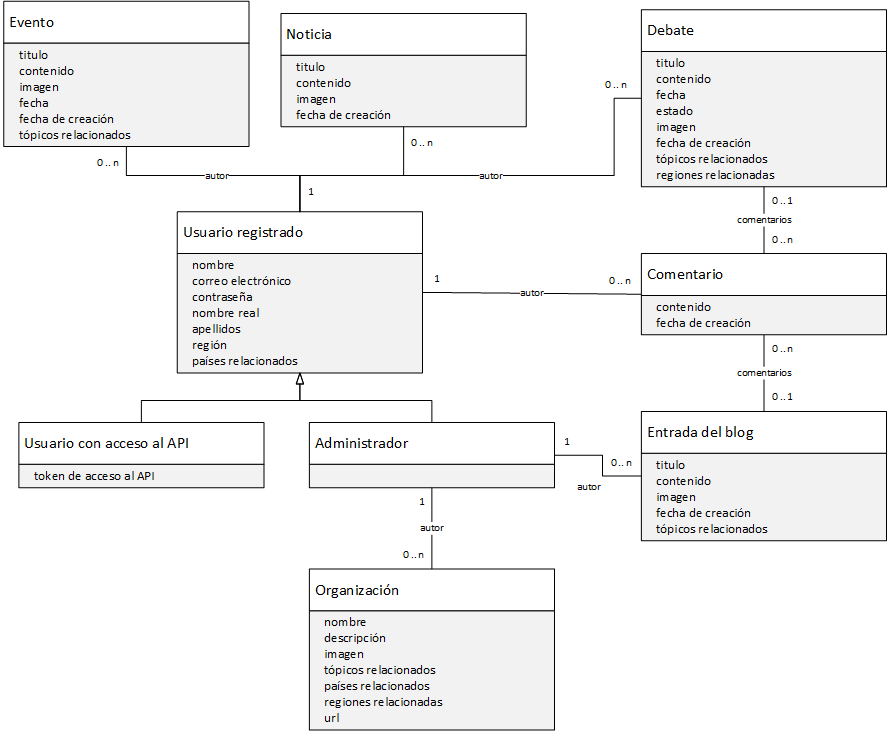
\includegraphics[height=\textwidth]{clases/clases_debate_preliminar}
		\caption{Diagrama de clases preliminares de la zona social}
		\label{fig:clases_preliminares_modelo_debate}
	\end{figure}
\end{landscape}

\subsubsection{Descripción de las clases}
\begin{description}
\item[Usuario registrado]	Representa a los usuarios que tienen una cuenta de usuario y han iniciado sesión en el portal.  Puede crear noticias, eventos, debates y realizar comentarios.  Sus atributos son los siguientes:
							\begin{itemize}
								\item \textbf{Nombre}  Será el nombre con el que el sistema identifica a cada usuario.  El nombre de usuario debe ser único.
								\item \textbf{Correo electrónico}  Será la dirección a la que el sistema enviará los correos electrónicos de contacto, por ejemplo: cuando el usuario solicita una nueva contraseña.  El correo electrónico debe ser único.
								\item \textbf{Contraseña}  Será utilizada para autenticar la identidad del usuario al iniciar sesión en el sistema o al modificar la información de su perfil.
								\item \textbf{Nombre real}  Será el nombre real del usuario, podrá ser visto por otros usuarios al visitar su perfil.
								\item \textbf{Apellidos}  Serán los apellidos reales del usuario, podrán ser vistos por otros usuarios al visitar su perfil.
								\item \textbf{Continente}  Será el continente en el que se encuentra el usuario.  Éste atributo no será obligatorio y podrá estar vacío.
								\item \textbf{Países relacionados}  Serán los países en los que el usuario tiene algún tipo de interés.  Este atributo no será obligatorio y podrá estar vacío.
							\end{itemize}
\item[Usuario con acceso al API]  Representa a los usuarios registrados que tienen capacidad de acceso al API del sistema.  Tienen las mismas capacidades que cualquier usuario registrado.  Además de los atributos de cualquier usuario registrado también tendrán:
							\begin{itemize}
							\item \textbf{Token}  Será la clave con la que el usuario accede al API.  Ésta clave será secreta y no podrá ser vista por ningún otro usuario.
							\end{itemize}
\item[Administrador]  Representa a los usuarios registrados con privilegios de administración en el sistema.  Tendrán los mismos atributos que cualquier otro usuario registrado pero podrán crear, modificar y eliminar cualquier contenido o comentario.
\item[Noticia]  Representa una noticia de interés en la que la fecha no es importante.  Las noticias podrán ser creadas por cualquier usuario registrado.  Sus atributos serán los siguientes:
							\begin{itemize}
							\item \textbf{Título}  Es el título de la noticia.
							\item \textbf{Contenido}  Es el contenido de la noticia.
							\item \textbf{Imagen}  Es una imagen relacionada con el contenido de la noticia.  Éste atributo no será obligatorio y podrá estar vacío.
							\item \textbf{Fecha de creación}  Es la fecha en la que la noticia fue creada.  Este campo es almacenado automáticamente por el sistema.
							\item \textbf{Autor}  Es el usuario registrado que crea la noticia.  Cada noticia tendrá un único autor, pero cada usuario registrado podrá ser autor de múltiples noticias.
							\end{itemize}
\item[Evento]  Representa una situación o noticia que tendrá lugar en un determinado momento del tiempo.  Los eventos podrán ser creados por cualquier usuario registrado.  Sus atributos serán los siguientes:
							\begin{itemize}
							\item \textbf{Título}  Es el título del evento.
							\item \textbf{Contenido}  Es el contenido del evento, donde se explica toda la información necesaria.
							\item \textbf{Imagen}  Es una imagen relacionada con el contenido del evento.  Éste atributo no será obligatorio y podrá estar vacío.
							\item \textbf{Fecha}  Será la fecha en la que el evento tendrá lugar.
							\item \textbf{Fecha de creación}  Es la fecha en la que el evento fue creado.  Este campo es almacenado automáticamente por el sistema.
							\item \textbf{Tópicos relacionados}  Serán los tópicos relacionados con el contenido del evento.  Los tópicos servirán como metainformación sobre el contenido y ayudarán a enriquecer los resultados de la búsqueda.
							\item \textbf{Autor}  Es el usuario registrado que crea el evento.  Cada evento tendrá un único autor, pero cada usuario registrado podrá ser autor de múltiples eventos.
							\end{itemize}
\item[Debate]  Representa un tema u opinión en el que se quiere permitir la participación de los usuarios.  Sus atributos serán los siguientes:
							\begin{itemize}
							\item \textbf{Título}  Es el título del debate.
							\item \textbf{Contenido}  Es el contenido del debate, donde se expone el tema a tratar por los usuarios.
							\item \textbf{Fecha}  Será la fecha o periodo de fechas en las que el debate tendrá lugar.
							\item \textbf{Estado}  Es el estado en el que se encuentra el debate.  Los posibles estados son ``abierto'', ``cerrado'' o ``próximamente''.
							\item \textbf{Imagen}  Es una imagen relacionada con el contenido del debate.  Éste atributo no será obligatorio y podrá estar vacío.
							\item \textbf{Fecha de creación}  Es la fecha en la que el debate fue creado.  Este campo es almacenado automáticamente por el sistema.
							\item \textbf{Tópicos relacionados}  Serán los tópicos relacionados con el contenido del debate.  Los tópicos servirán como metainformación sobre el contenido y ayudarán a enriquecer los resultados de la búsqueda.
							\item \textbf{Regiones relacionadas}  Serán las regiones relacionadas con el debate o a las que éste hace referencia.  Al igual que los tópicos, las regiones servirán como metainformación sobre el contenido y ayudarán a enriquecer los resultados de la búsqueda.
							\item \textbf{Autor}  Es el usuario registrado que crea el debate.  Cada debate tendrá un único autor, pero cada usuario registrado podrá ser autor de múltiples debates.
							\item \textbf{Comentarios}  Son los comentarios que los usuarios realizan en el debate.  Cada debate podrá tener múltiples comentarios, pero cada comentario sólo podrá pertenecer a un debate.
							\end{itemize}
\item[Entrada del blog]  Representa una entrada en el blog oficial de Land Portal.  Las entradas en el blog sólo pueden ser creadas por los administadores.  Sus atributos son los siguientes:
							\begin{itemize}
							\item \textbf{Título}  Es el título de la entrada.
							\item \textbf{Contenido}  Es el contenido de la entrada.
							\item \textbf{Imagen}  Es una imagen relacionada con el contenido de la entrada.  Éste atributo no será obligatorio y podrá estar vacío.
							\item \textbf{Fecha de creación}  Es la fecha en la que la entrada fue creada.  Este campo es almacenado automáticamente por el sistema.
							\item \textbf{Tópicos relacionados}  Serán los tópicos relacionados con el contenido de la entrada.  Los tópicos servirán como metainformación sobre el contenido y ayudarán a enriquecer los resultados de la búsqueda.
							\item \textbf{Autor}  Es el administrador que crea la entrada.  Cada entrada tendrá un único autor, pero cada administrador podrá ser autor de múltiples entradas.
							\item \textbf{Comentarios}  Son los comentarios que los usuarios realizan en la entrada.  Cada entrada podrá tener múltiples comentarios, pero cada comentario sólo podrá pertenecer a una entrada.
							\end{itemize}
\item[Comentario]  Representa la opinión que un usuario hace pública en un debate o una entrada del blog:
							\begin{itemize}
							\item \textbf{Contenido}  Es el contenido del comentario.
							\item \textbf{Fecha de creación}  Es la fecha en la que el comentario fue creado.  Este campo es almacenado automáticamente por el sistema.
							\item \textbf{Autor}  Es el usuario registrado que crea el comentario.  Cada comentario tiene un autor, pero un usuario registrado puede ser autor de múltiples comentarios.
							\end{itemize}
\end{description}


\section{Análisis de interfaces de usuario}
\label{analisis_interfaces_usuario}
En esta sección se realizará una primera aproximación a la posible interfaz que tendrá el portal, detallando y explicando las vistas que la conforman.  A continuación se mostrarán los \textit{mockups} de la interfaz y se explicará cada uno de ellos.



\subsection{Interfaz de la zona de datos}
Como se ha mencionado en la sección ``\nameref{definicion_sistema}'' perteneciente al capítulo \ref{chapter04}, la interfaz de zona de datos (o \textit{LandBook}) queda fuera del alcance de éste proyecto, por lo que no se mostrarán \textit{mockups} para dicha sección.



\subsection{Interfaz de administración}
La interfaz de administración será directamente proveída por el gestor de contenidos que, como se ha mencionado en la sección ``\nameref{chapter02:alternativas_seleccionadas}'' perteneciente al capítulo \ref{chapter02}, será Drupal.  Por esta razón no se mostrarán \textit{mockups} pertenecientes a dicha interfaz.



\subsection{Interfaz de la zona social}
A continuación se mostrarán los \textit{mockups} de la zona social (o \textit{LandDebate}).


\subsubsection{Vista del blog del Land Portal}
\label{chapter04:mockup_blog}
La figura \ref{fig:mockup_blog} muestra el \textit{mockup} de la vista que conformará el blog del nuevo Land Portal.

Ésta pantalla mostrará las entradas del blog ordenadas de más a menos reciente.  Las tres entradas más recientes se destacarán sobre el resto, e incluirán:
\begin{itemize}
	\item Título de la entrada, enlazado a la vista de detalle de la propia entrada.
	\item Imagen de la entrada.
	\item Autor y fecha en la que la entrada fue añadida al blog.
	\item Tópicos relacionados.  Al pulsar en un tópico, se accederá a una vista en la que se mostrarán todos los contenidos del portal relacionados con dicho tópico.
	\item Resumen del contenido de la entrada.
\end{itemize}

\begin{figure}[h]
	\centering
	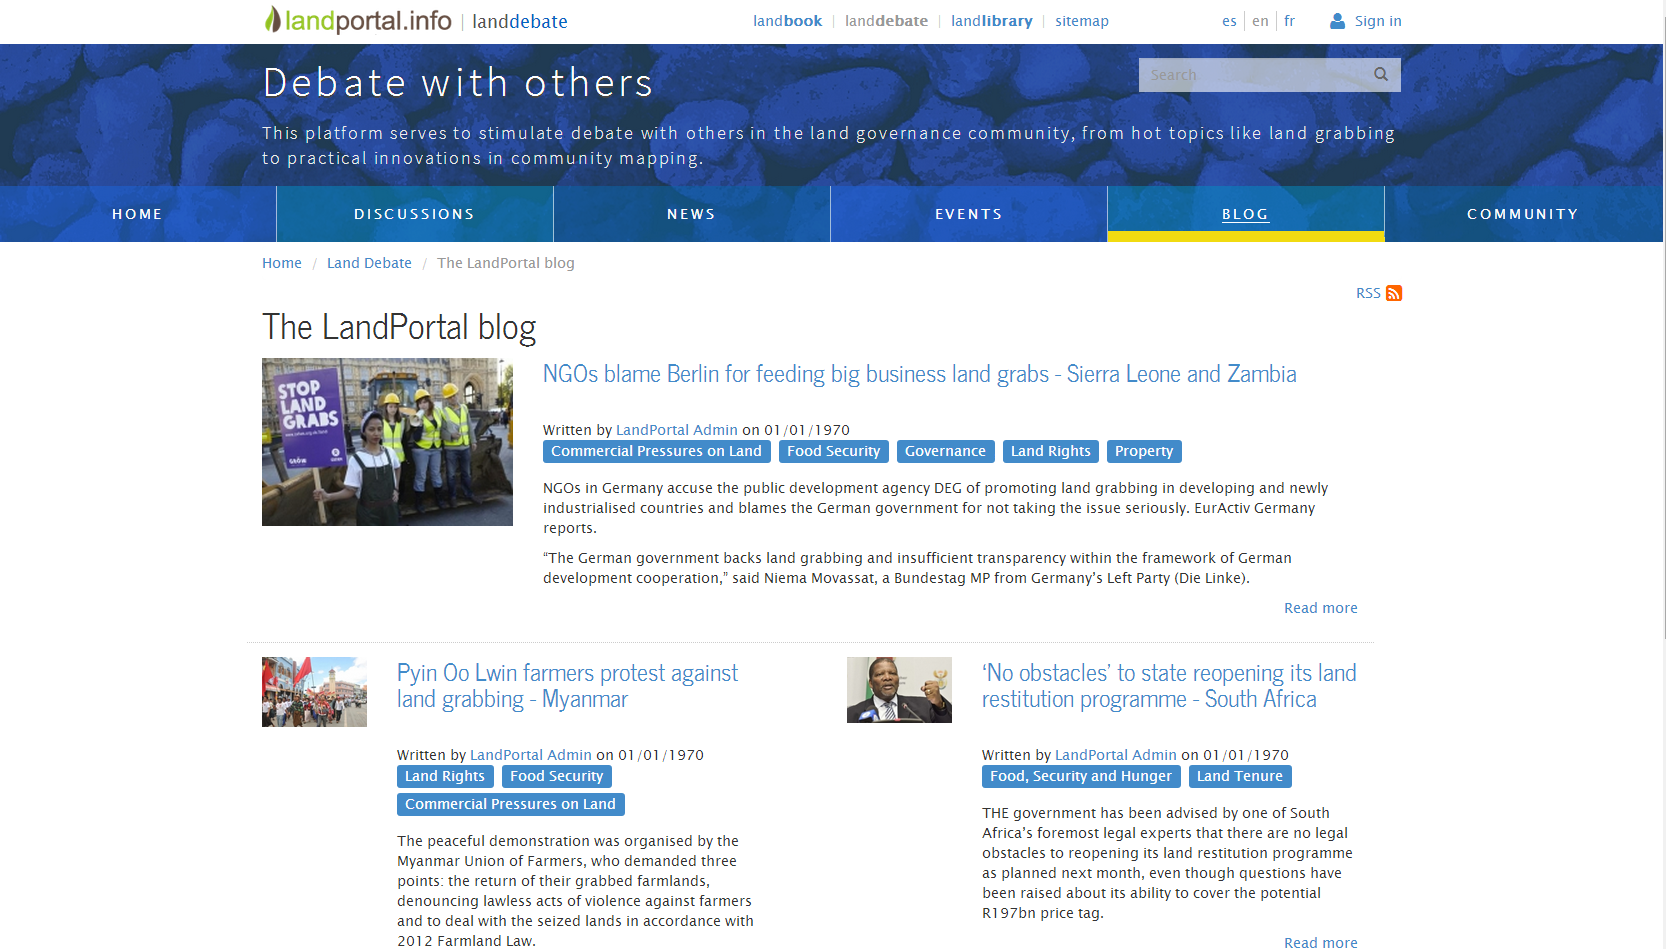
\includegraphics[width=\textwidth]{mockups/blog}
	\caption{\textit{Mockup} de la vista del blog del Land Portal}
	\label{fig:mockup_blog}
\end{figure}

Las entradas anteriores tendrán menos énfasis en la vista, y sólo estarán representadas por su título y la fecha en la que han sido creadas.  Además también se incluirá un paginador para recorrer las noticias anteriores y un enlace al \textit{feed} RSS\footnote{El feed RSS permite suscribirse a las últimas entradas del blog utilizando un lector de feeds RSS como Feedly, Newsvibe o Digg Reader y obtener las actualizaciones de forma automática en el lector sin necesidad de acceder al portal.} donde también se encontrarán las últimas noticias.


\subsubsection{Vista de detalle de una entrada del blog}
\label{chapter04:mockup_blog_entry}
La figura \ref{fig:mockup_entrada_blog} muestra el \textit{mockup} de la vista de detalle de una entrada del blog.  Esta vista incluirá:
\begin{itemize}
	\item Título de la entrada
	\item Autor y fecha de creación de la entrada
	\item Tópicos relacionados.  Como ya se ha explicado anteriormente, al pulsar sobre un tópico, el sistema cargará una vista con todos los contenidos relacionados con dicho tópico.
	\item Contenido de la entrada
	\item Imagen relacionada
	\item Botones destinados a compartir el contenido de la entrada en redes sociales como Twitter o Facebook.
\end{itemize}

En la zona inferior de la vista se incluirá la sección de comentarios.  En esta sección los usuarios podrán participar y dar su opinión a cerca del tema tratado en la entrada del blog.  Cada comentario mostrará su contenido, su autor y la fecha en al que fue creado.  Los comentarios se mostrarán ordenados según su fecha de creación.

\begin{figure}[h]
	\centering
	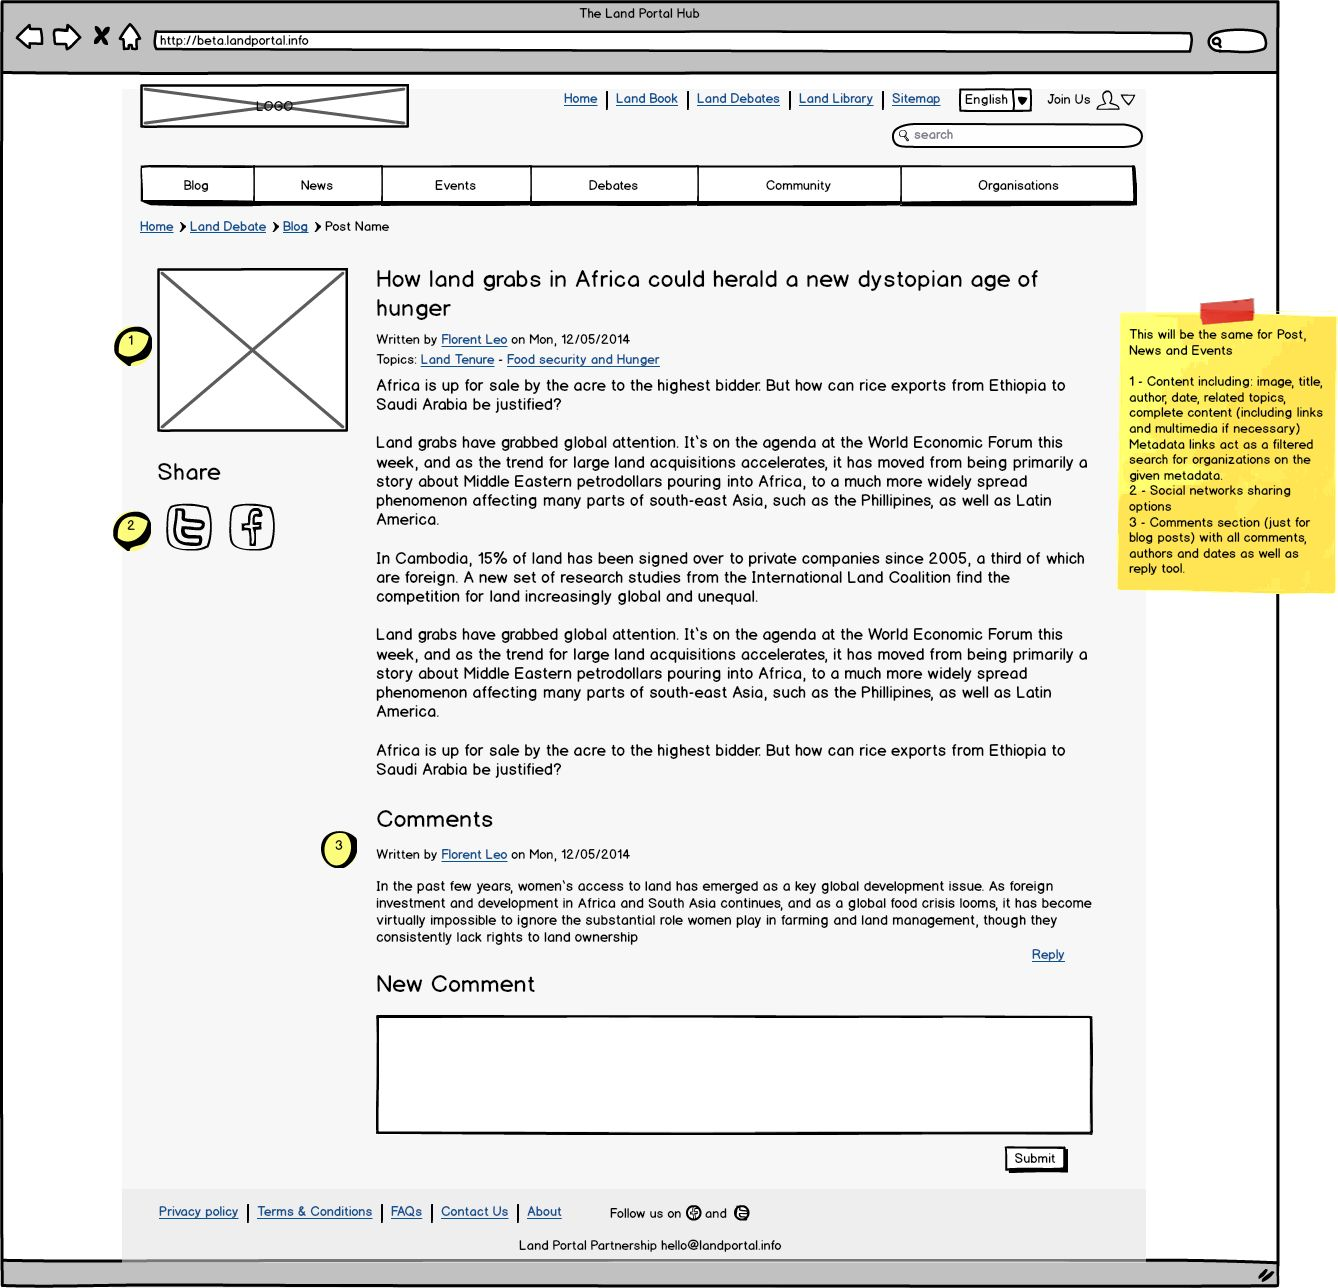
\includegraphics[width=\textwidth]{mockups/post-new-event}
	\caption{\textit{Mockup} de la vista de detalle de una entrada del blog}
	\label{fig:mockup_entrada_blog}
\end{figure}


\subsubsection{Vista de eventos}
\label{chapter04:mockup_eventos}
La figura \ref{fig:mockup_eventos} muestra el \textit{mockup} de la vista de eventos del nuevo Land Portal.  Los dos eventos más recientes se destacarán sobre el resto e incluirán:
\begin{itemize}
	\item Título del evento, enlazado a la vista de detalle del propio evento.
	\item Imagen del evento.
	\item Autor y fecha en la que el evento fue creado.
	\item Tópicos relacionados.  Al pulsar en un tópico, se accederá a una vista en la que se mostrarán todos los contenidos del portal relacionados con dicho tópico.
	\item Resumen del contenido del evento.
\end{itemize}
De forma similar a como sucede en el blog, los eventos anteriores tendrán menos importancia en la vista, y únicamente se mostrarán con su título y la fecha en la que el evento tiene lugar.  También al igual que el blog, se incluye un paginador y un enlace al \textit{feed} RSS donde también se encontrarán los últimos eventos.

Un añadido especial de ésta vista es un calendario que mostrará resaltados los días en los que tiene lugar algún evento.
\begin{figure}[h]
	\centering
	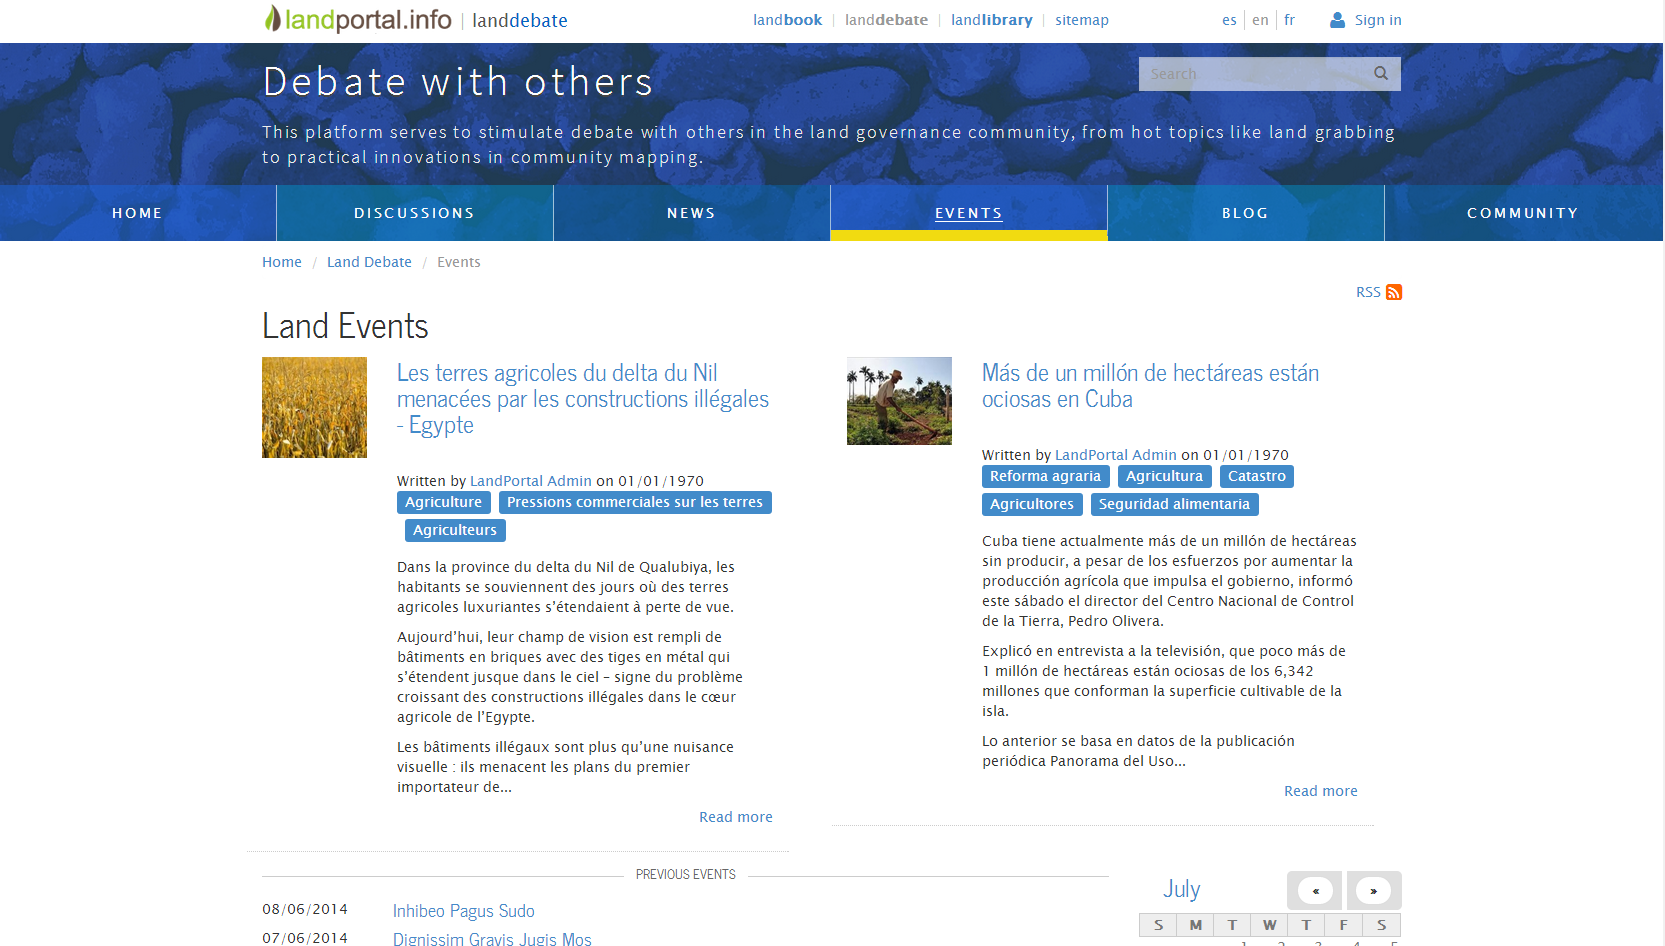
\includegraphics[width=\textwidth]{mockups/events}
	\caption{\textit{Mockup} de la vista de eventos}
	\label{fig:mockup_eventos}
\end{figure}


\subsubsection{Vista de noticias}
\label{chapter04:mockup_noticias}
La figura \ref{fig:mockup_noticias} muestra el \textit{mockup} de la vista de noticias del nuevo Land Portal.  Las cuatro noticias más recientes se destacarán sobre el resto e incluirán:
\begin{itemize}
	\item Título de la noticia, enlazado a la vista de detalle de la propia noticia.
	\item Imagen de la noticia
	\item Resumen del contenido de la noticia.
\end{itemize}
Al igual que en la vista de eventos y del blog, las noticias anteriores sólo mostrarán su título y fecha de creación.  También se incluirán, de la misma forma que las vistas anteriores, un paginador y un enlace al \textit{feed} RSS con las últimas noticias.

Una característica especial de ésta vista será que en la parte izquierda de la misma se mostrarán las últimas actualizaciones de la cuenta de Twitter de Land Portal\footnote{La cuenta oficial de Land Portal se puede ver en \url{https://twitter.com/landportal}}.  Para incluír éste componente se utilizará la capacidad de generación de \textit{widgets} de Twitter.
\begin{figure}[h]
	\centering
	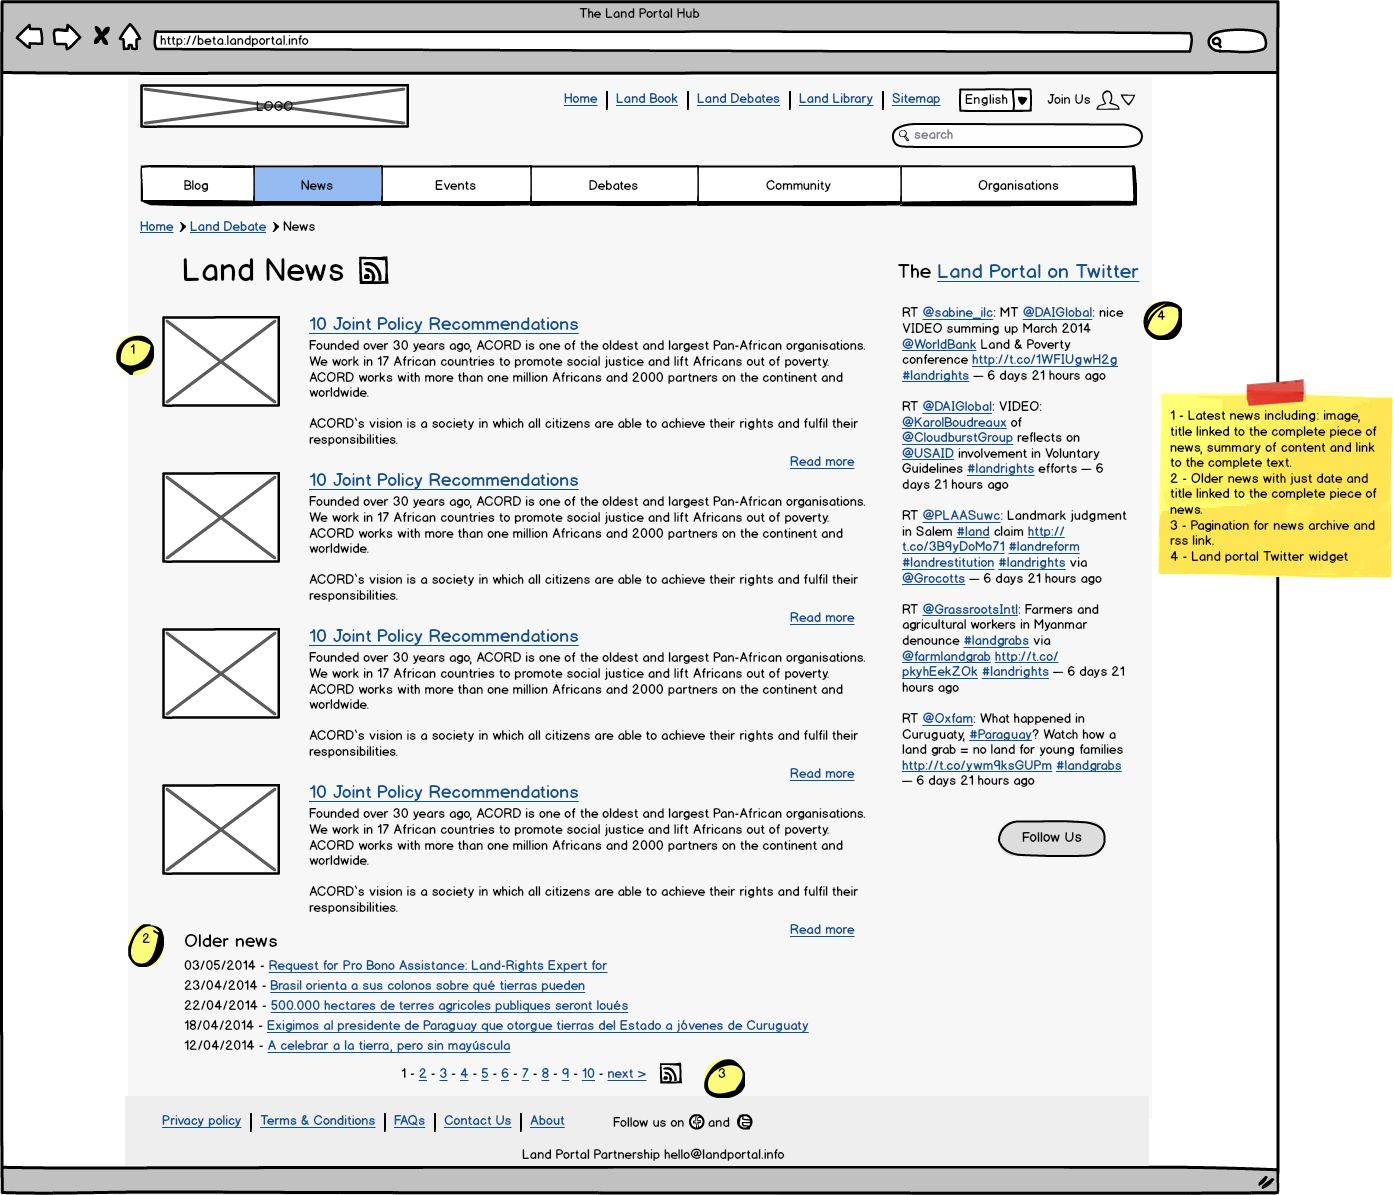
\includegraphics[width=\textwidth]{mockups/news}
	\caption{\textit{Mockup} de la vista de noticias}
	\label{fig:mockup_noticias}
\end{figure}


\subsubsection{Vista de debates}
La figura \ref{fig:mockup_debates} muestra el \textit{mockup} de la vista de debates del nuevo Land Portal.  Ésta vista tiene una importancia clave dentro de la zona social, puesto que los debates serán el principal punto en el que los usuarios participen e intercambien opiniones.  Los debates que no estén cerrados se destacarán sobre el resto e incluirán:
\begin{itemize}
	\item Título del debate, enlazado a la vista de detalle del mismo.
	\item Autor del debate.
	\item Tópicos relacionados.  Al pulsar en un tópico, se accederá a una vista en la que se mostrarán todos los contenidos del portal relacionados con dicho tópico.
	\item Resumen del contenido del debate.
	\item Imagen del debate.
	\item Fecha o fechas en las que el debate tendrá lugar.
	\item Estado del debate.
\end{itemize}

De forma similar a las vistas anteriores, también se incluirán los debates anteriores (en este caso los debates ya cerrados) únicamente con su título y la fecha en la qu ese han creado y un enlace al \textit{feed} RSS de la sección de debates.

Puesto que, como se ha dicho anteriormente, ésta vista juega un papel clave fomentando la participación de los usuarios en el portal.  Por ello, en la zona derecha se mostrarán los últimos comentarios que los usuarios hayan realizado en algún debate.  Cada comentario incluirá:
\begin{itemize}
	\item Fecha de creación del comentario.
	\item Autor del comentario.
	\item Título del comentario enlazado al propio comentario dentro de la vista de detalle del debate.
	\item Resumen del contenido del comentario.
\end{itemize}
\begin{figure}[h]
	\centering
	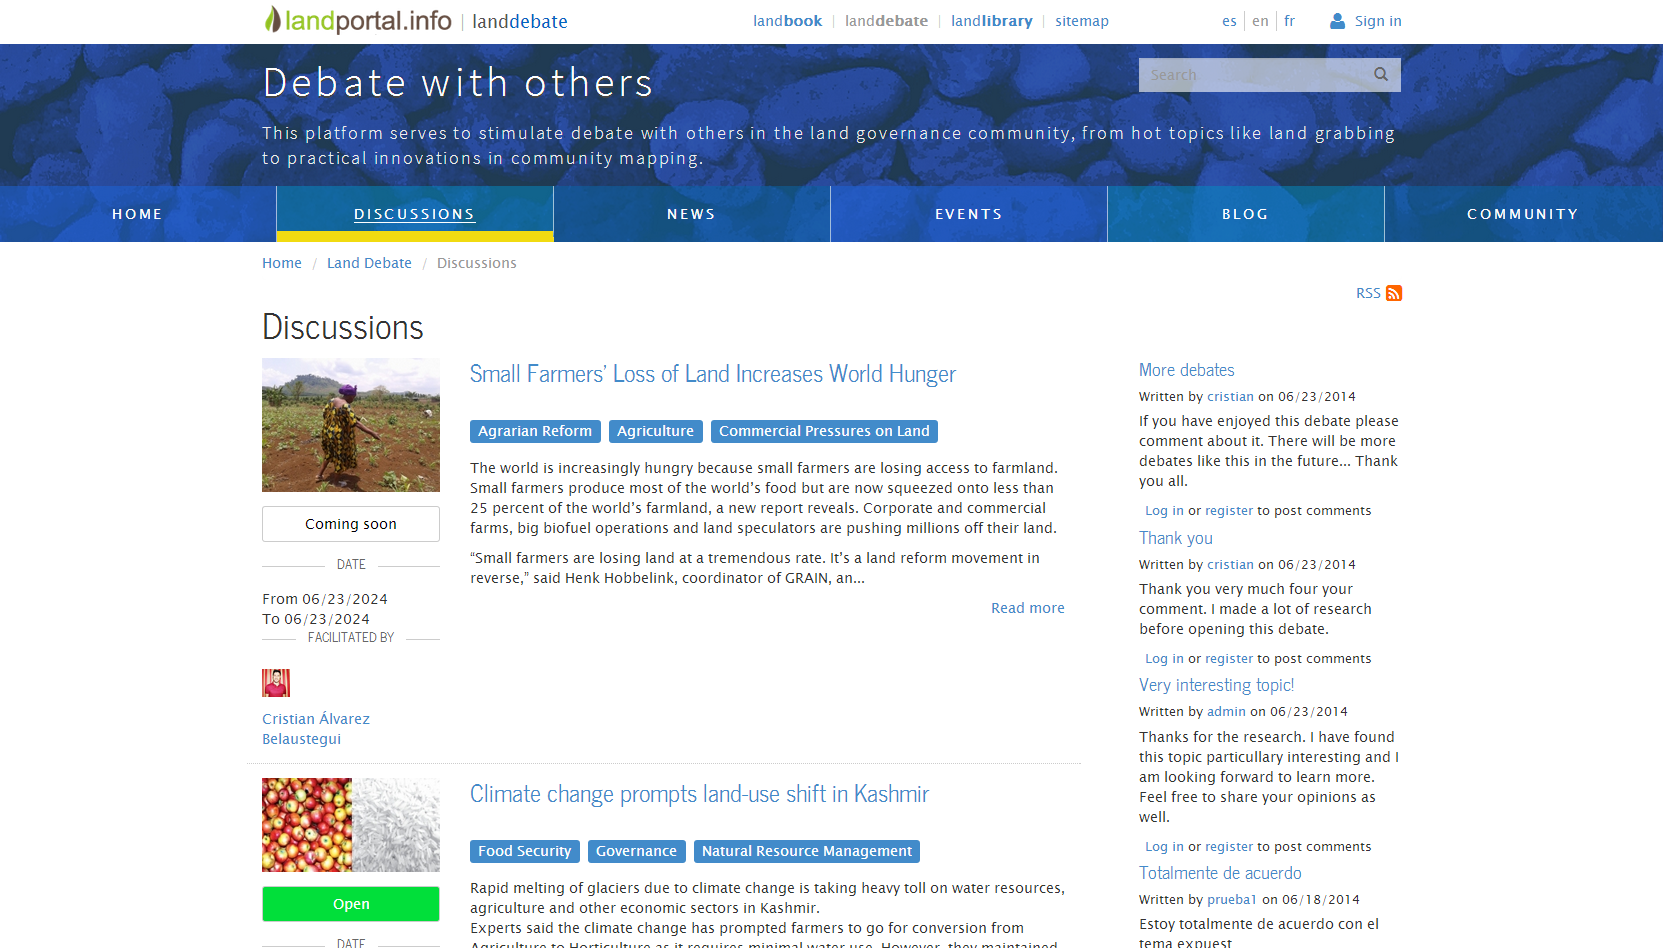
\includegraphics[width=\textwidth]{mockups/debates}
	\caption{\textit{Mockup} de la vista de debates}
	\label{fig:mockup_debates}
\end{figure}


\subsubsection{Vista de detalle de un debate}
La figura \ref{fig:mockup_debate} muestra el \textit{mockup} de la vista de detalle de un debate.  Al igual que la vista de debates descrita anteriormente, esta vista juega también un rol clave para fomentar la participación de los usuarios en el portal.

La vista incluirá toda la información del debate, incluyendo:
\begin{itemize}
	\item Título del debate
	\item Tópicos y países relacionados
	\item Idioma en el que tendrá lugar el debate
	\item Contenido del debate
	\item Imagen del debate
	\item Estado
	\item Autor del debate
\end{itemize}

En la parte inferior de esta vista se ubicará la sección de comentarios.  El comportamiento de la sección de comentarios variará en función del estado del debate.  Cuando el debate esté abierto, los usuarios podrán participar e incluir nuevos comentarios o  responder a los comentarios ya existentes.  Cuando el debate esté cerrado se mostrarán los comentarios existentes, pero no se permitirá añadir ningún comentario nuevo.  Los comentarios se mostrarán ordenados según su fecha de creación.

Para reforzar la función social de esta vista, se incluirán también una serie de botones que permitirán compartir el debate en redes sociales como Twitter o Facebook.  Al mismo tiempo, en la parte derecha de la vista se mostrarán los últimos comentarios relacionados en la red social Twitter.

\begin{figure}[h]
	\centering
	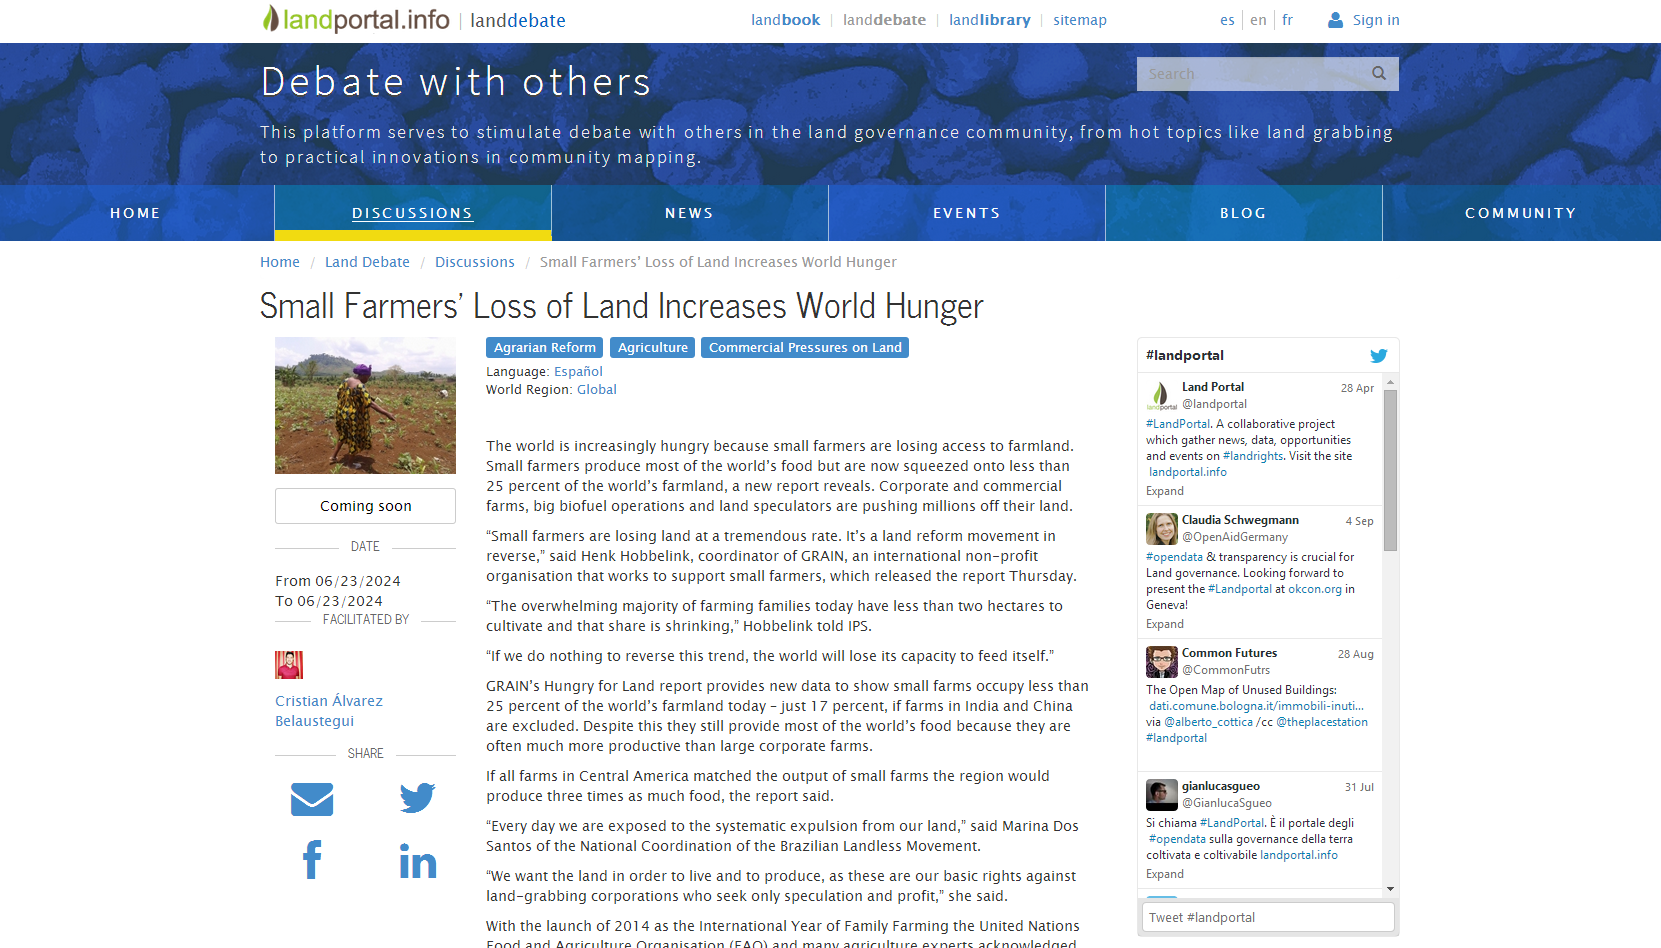
\includegraphics[width=\textwidth]{mockups/debate}
	\caption{\textit{Mockup} de la vista de detalle de un debate}
	\label{fig:mockup_debate}
\end{figure}


\subsubsection{Vista de detalle de un evento y de una noticia}
\label{mockup_noticia_evento}
Las vistas del detalle de un evento y una noticia serán similares a la vista de detalle de una entrada en el blog, el \textit{mockup} para dicha vista puede verse en la figura \ref{fig:mockup_entrada_blog}.

La única diferencia de estas vistas respecto a la vista de detalle de una entrada del blog será que ni los eventos ni las noticias tendrán sección de comentarios.


\subsubsection{Vista de organizaciones}
La figura \ref{fig:mockup_organizaciones} muestra el \textit{mockup} de la vista de organizaciones. Esta vista mostrará las organizaciones existentes en el portal en forma de parrilla o \textit{grid}, en la que cada organización mostrará su imagen y su nombre, ambos enlazados a la vista de detalle de dicha organización.

En la zona derecha de la vista se incluirán una serie de controles con los que será posible buscar organizaciones determinadas.  Además, siguiendo con la tónica social del portal ya mencionada anteriormente, se mostrará un \textit{widget} con el contenido de la comunidad de Land Portal en la red social Facebook\footnote{La página oficial de Land Portal en Facebook puede verse en la siguiente dirección: \url{https://www.facebook.com/landportal}}.

\begin{figure}[h]
	\centering
	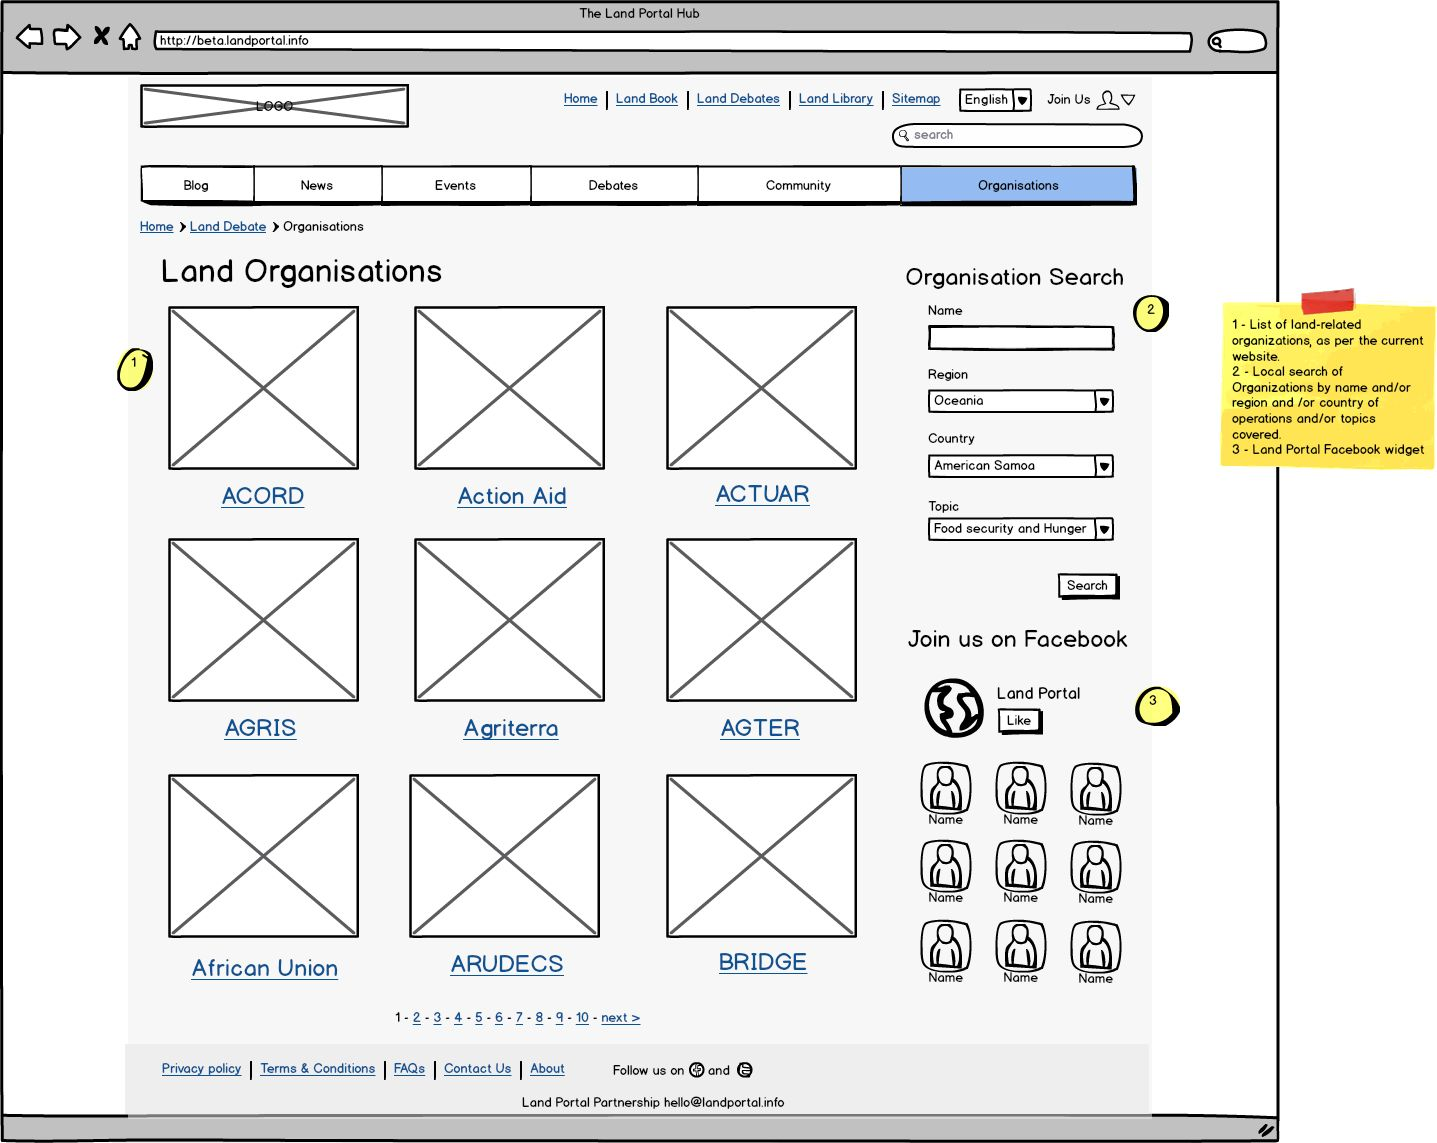
\includegraphics[width=\textwidth]{mockups/organisations}
	\caption{\textit{Mockup} de la vista de organizaciones}
	\label{fig:mockup_organizaciones}
\end{figure}


\subsubsection{Vista de detalle de una organización}
La figura \ref{fig:mockup_organizacion} muestra el \textit{mockup} de la vista de detalle de una organización. Esta vista mostrará las organizaciones existentes en el portal en forma de parrilla o \textit{grid}, en la que cada organización mostrará su imagen y su nombre, ambos enlazados a la vista de detalle de dicha organización.

Esta vista mostrará la imagen, el nombre y una descripción de la organización.  Además también se incluirá un enlace a la página web de dicha organización.  En la parte derecha de la vista se mostrarán los metadatos de la organización, como: el área y los países en los que opera o los tópicos relacionados.  Al pulsar en cualquier término de estos metadatos el sistema cargará una vista que mostrará todo el contenido del portal relacionado con dicho término.

\begin{figure}[h]
	\centering
	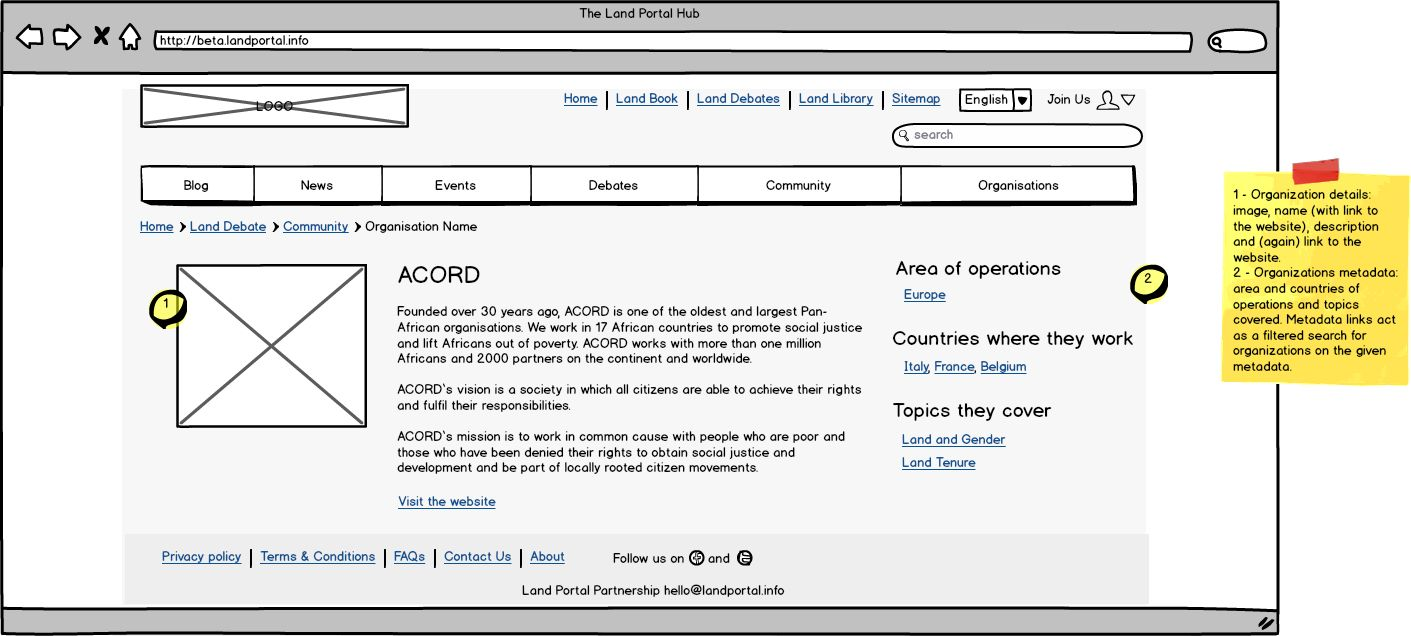
\includegraphics[width=\textwidth]{mockups/organisation}
	\caption{\textit{Mockup} de la vista de detalle de una organización}
	\label{fig:mockup_organizacion}
\end{figure}


\subsubsection{Vista de comunidad}
La vista de la comunidad será similar a la vista de organizaciones, la cual se puede ver en la figura \ref{fig:mockup_organizaciones}.  Las únicas diferencias respecto a la vista de organizaciónes serán:
\begin{itemize}
	\item En lugar de mostrar las organizaciones del portal, esta vista mostrará en una parrilla o \textit{grid} los usuarios registrados en el portal.
	\item En la zona derecha (además del formulario de búsqueda y el \textit{widget} de la red social Facebook) se incluirá un botón para facilitar el registro de nuevos usuarios.
\end{itemize}

\subsubsection{Vista de login}
La figura \ref{fig:mockup_login} muestra el \textit{mockup} de la vista de login. Esta vista permitirá que los usuarios inicien sesión en el portal.  La vista de login contará con un formulario donde el usuario introducirá su nombre de usuario o email y su contraseña para iniciar sesión en el sistema.  También existirá un enlace mediante el cual un usuario podrá solicitar una nueva contraseña en caso de haber olvidado la suya.

Además, siguiendo con la línea social del portal, se incluyen dos botones destinados a iniciar sesión en el sistema utilizando las redes sociales Twitter y Facebook.

\begin{figure}[h]
	\centering
	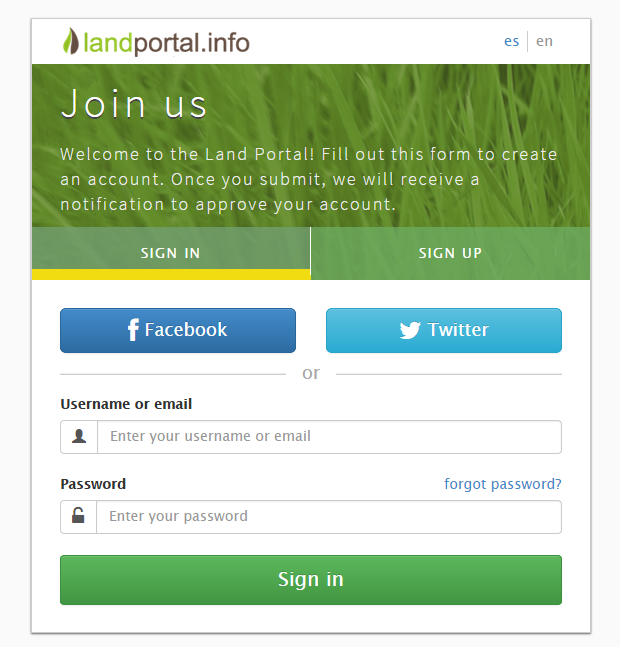
\includegraphics[width=\textwidth]{mockups/login}
	\caption{\textit{Mockup} de la vista de login}
	\label{fig:mockup_login}
\end{figure}


\subsubsection{Vista de registro}
La figura \ref{fig:mockup_registro} muestra el \textit{mockup} de la vista de registro. Esta vista permitirá a los usuarios crear una nueva cuenta en el sistema.  La vista de registro contará con un formulario donde el usuario introducirá su nombre de usuario, su email, su nombre y apellidos y los países y continentes en los que esté interesado. Los campos obligatorios para crear una nueva cuenta de usuario están marcados con un asterisco.  

El botón de registro creará la nueva cuenta en el sistema con un estado ``desactivado'', a la espera de ser activada por un administrador.

\begin{figure}[h]
	\centering
	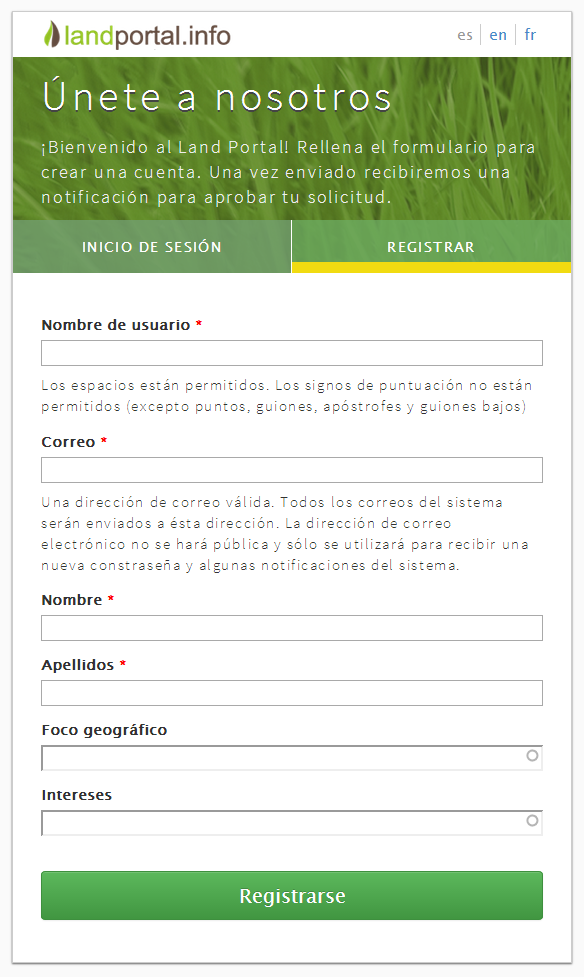
\includegraphics[width=\textwidth]{mockups/register}
	\caption{\textit{Mockup} de la vista de registro}
	\label{fig:mockup_registro}
\end{figure}




\subsubsection{Vista de búsqueda}
La figura \ref{fig:mockup_buscar} muestra el \textit{mockup} de la vista de búsqueda.  Esta vista permitirá a los usuarios buscar cualquier tipo de contenido en el portal.   Al pulsar sobre cada resultado de búsqueda el usuario accederá a la vista de detalle del mismo.

Como se puede ver en la imagen, cada resultado de la búsqueda se presentará de una forma diferente y tendrá asociada una etiqueta en la que se indica el tipo de contenido al que pertenece.  Al pulsar en esta etiqueta, el sistema cargará la vista correspondiente a cada tipo de contenido.

\begin{figure}[h]
	\centering
	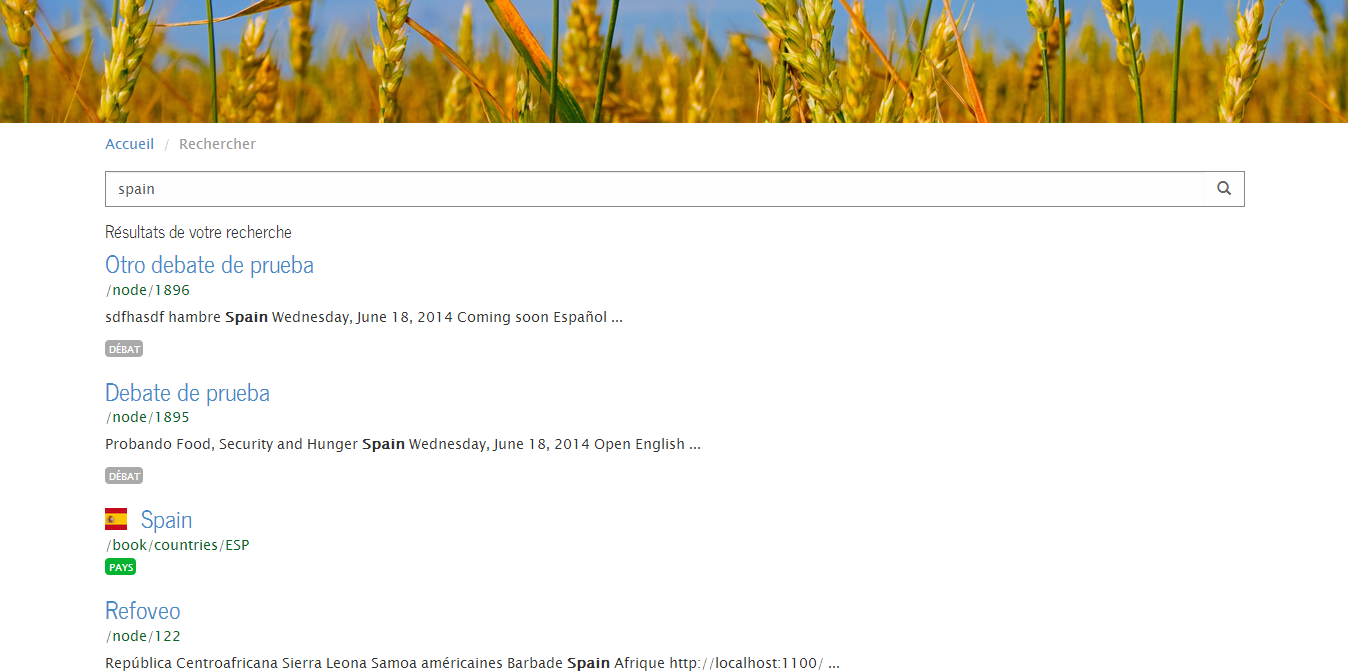
\includegraphics[width=\textwidth]{mockups/search}
	\caption{\textit{Mockup} de la vista de busqueda}
	\label{fig:mockup_buscar}
\end{figure}


\section{Especificación del plan de pruebas}
\label{especificacion_plan_pruebas}
En esta sección se especificará el plan de pruebas que se seguirá durante el desarrollo del proyecto.  Se detallará que tipos de pruebas se realizarán, sobre qué componentes y en qué momento del desarrollo tendrán lugar.


\subsection{Pruebas unitarias}
Las pruebas unitarias están dirigidas a probar partes de código pequeñas y específicas. Como Martin Fowler explica en su artículo \cite{mfowler:unit-testing} existen tres características fundamentales que caracterizan a las pruebas unitarias:
\begin{itemize}
	\item Los tests se centran en una parte pequeña del sistema
	\item Los tests son normalmente escritos por los propios programadores utilizando alguna variante del framework \textit{XUnit}\footnote{XUnit es el nombre que recibe una familia de frameworks destinados a la realización de pruebas.  El primero de éstos frameworks fue creado por Kent Beck para el lenguaje Smalltalk.  Para más información al respecto se recomienda el artículo \cite{mfowler:xunit}.}.
	\item Se espera que los tests se ejecuten de una forma rápida
\end{itemize}

Un punto clave de las pruebas unitarias es su aislamiento de otras partes del sistema.  Por la estructura del subsistema de datos, cuya principal funcionalidad es insertar y extraer valores de la base de datos, sería necesario crear una gran cantidad de \textit{mocks} que simulen el funcionamiento de la propia base de datos.  Debido a esto, se ha tomado la decisión de no realizar pruebas unitarias como tal, puesto que supondría un sobreesfuerzo muy grande aislar totalmente los componentes del subsistema de la base de datos para obtener un coste muy pequeño, puesto que la propia base de datos juega un punto clave en el correcto funcionamiento de éste subsistema.

Por su construcción que, como ya se ha mencionado en secciones anteriores, delega la funcionalidad principal a los mecanismos proveídos por el gestor de contenidos, las pruebas unitarias se omitirán para la zona social y los subsistemas que engloba.

\subsection{Pruebas de integración}
A pesar de lo mencionado anteriormente a cerca de las pruebas unitarias, existen opiniones divididas sobre lo que se considera exactamente una \textit{unidad} en dichas pruebas.  Para éste proyecto, y hablando del subsistema de datos, se tomará como una \textit{unidad} la lectura de un valor del fichero XML y su inmediata inserción en la base de datos.\newline
Según la opinión de diferentes autores (entre ellos el propio Martin Fowler, como menciona en su artículo \cite{mfowler:unit-testing}), éste tipo de pruebas podrían ser consideradas pruebas unitarias.  No obstante, con el objetivo de mantener la máxima fidelidad respecto a la definición de pruebas unitarias, las pruebas que se detallan a continuación han sido finalmente consideradas como pruebas de integración.

Para el desarrollo del subsistema de datos se utilizará una metodología de Desarrollo Dirigido por Pruebas (o TDD)\footnote{El desarrollo dirigido por pruebas es una metodología de desarrollo de software creada por Kent Beck en 1990.  Para más información al respecto, se recomienda el libro ``Test Driven Development'' \cite{kbeck:test-driven-development}}.  Con el objetivo de facilitar ésta metodología se utilizará también un servidor de integración continua.

Debido al carácter de los subsistemas de la zona social, cuya principal funcionalidad queda delegada al núcleo del CMS, las pruebas para estos componentes tendrán lugar en forma de casos de prueba que se ejecutarán manualmente durante el desarrollo.  

El resultado de ambas pruebas podrá verse con mayor detalle en el capítulo \ref{chapter:desarrollo_pruebas} titulado ``\nameref{chapter:desarrollo_pruebas}''.


\subsection{Pruebas de aceptación}
Las pruebas de aceptación consisten en comprobar que el sistema realizado satisface las necesidades del usuario y el usuario \textit{acepta} la solución creada.  Normalmente las pruebas de aceptación son realizadas por el cliente del sistema que se construye y tienen lugar en las últimas fases del desarrollo del sistema.  Las pruebas de aceptación funcionan como una verificación final de que el sistema cumple con los requisitos y funciona de una forma adecuada para los usuarios.
En éste proyecto las pruebas de aceptación se realizarán en forma de pruebas beta.

Las pruebas beta se realizarán durante la última fase de desarrollo.  Concretamente tendrán lugar a lo largo de una semana en la que se contará con un servidor especial en el cual se desplegará la última versión estable del sistema.  Este servidor estará continuamente disponible, el cliente accederá a dicho servidor, probará los diferentes aspectos del sistema y ofrecerá \textit{feedback} a los desarrolladores con aquellos posibles fallos o cuestiones que encuentre.

Una vez recibidos los reportes será tarea del jefe de proyecto filtrarlos y separar aquellos que son fallos reales o posibles mejoras de aquellos que no lo son, y será tarea del equipo de desarrollo arreglar los fallos encontrados para obtener una versión final del sistema.


\subsection{Pruebas de rendimiento}
Tal y como se ha mencionado en la sección \nameref{especificacion_requisitos_no_funcionales}, perteneciente al capítulo \ref{chapter04}, el punto de entrada de datos puede recibir conjuntos de datos de gran volumen.  Por esto será necesario realizar pruebas específicas de rendimiento para dicho componente, con el fin de asegurar su correcto comportamiento ante diferentes entradas de datos de diferentes tamaños.

Dos puntos clave en éste tipo de pruebas son: el rendimiento temporal y el rendimiento espacial.  El rendimiento temporal se refiere a la velocidad con la que el componente realiza su tarea.  El rendimiento espacial se refiere a la cantidad de memoria que el componente utiliza durante su funcionamiento.

El punto de entrada de datos es un componente del sistema que se ejecutará una vez cada varios meses, por lo que el rendimiento temporal del mismo no tendrá una gran importancia.  El rendimiento espacial, en cambio, si tendrá una importancia alta, puesto que el consumo de memoria deberá estar controlado para evitar fallos con la llegada de grandes volúmenes de datos.

Atendiendo a la famosa cita de Donald Knuth extraída de \cite{knuth:structuredprogramming}, las pruebas de rendimiento tendrán lugar en las últimas fases del desarrollo del punto de entrada de datos: \quote{``\textit{Premature optimization is the root of all evil (or at least most of it) in programming.}''} 


